%% LyX 1.6.9 created this file.  For more info, see http://www.lyx.org/.
%% Do not edit unless you really know what you are doing.
\documentclass[oneside,english]{amsart}
%\documentclass[oneside,english]{article}\usepackage[T1]{fontenc}
\usepackage[utf8]{inputenc}
\usepackage{amsmath,amssymb,graphicx}
\usepackage{amsthm}
\usepackage{graphicx}
\usepackage{siunitx}
\usepackage{tikz}
%\usepackage{subfigure}
%\usepackage{epsfig}
%\usepackage{color}
%%%%%%%%%%%%%%%%%%%%%%%%%%%%%%%%%%%%%%%%%%%%%%%%
\graphicspath{{./Images/}}
%usepackage[dvips]{color}
%%%%%%%%%%%%%%%%%%%%%%%%%%%%%%%%%%%%%%%%%%%%%%%%%%%%%
\usepackage[left=2.5cm,right=2.5cm,top=3cm,bottom=3cm]{geometry}
%%%%%%%%%%%%%%%%%%%%%%%%%%%%%%%%%%%%%%%%%%%%%%%%%%%
%\newcommand{\cal}{\mathcal}
\newcommand{\beq}{\begin{equation}}
\newcommand{\eeq}{\end{equation}}
%%%%%%%%%%%%%%%%%%%%%%%%%%%%%%%%%%%%%%%%%%%%%%%%%%%%%
\def\sinc{\mathop{\rm sinc}\nolimits}  
\def\cal{\mathop{\rm cal}\nolimits}  
\def\cal{\mathop{\rm cal}\nolimits}  
\def\CFL{\mathop{\rm CFL}\nolimits}  
\def\VDM{\mathop{\rm VDM}\nolimits}  
\def\RK4{\mathop{\rm RK4}\nolimits}  
\def\ex{\mathop{\rm ex}\nolimits}  
\def\atan{\mathop{\rm atan}\nolimits}  
\def\sech{\mathop{\rm sech}\nolimits}  
\def\tanh{\mathop{\rm tanh}\nolimits}  
\def\div{\mathop{\rm div}\nolimits}  
\def\deg{\mathop{\rm deg}\nolimits}  
\def\vort{\mathop{\rm curl}\nolimits}  
\def\vorth{\mathop{\rm curl}\nolimits}  
\def\days{\mathop{\rm days}\nolimits}  
\def\Re{\mathop{\rm Re}\nolimits}  
\def\Sp{\mathop{\rm Sp}\nolimits}  
\newcommand{\bgrad}{\mbox{\boldmath$\nabla$}}
\newcommand{\bnabla}{\mbox{\boldmath$\nabla$}}
\newcommand{\bA}{\mbox{\boldmath$A$}}
\newcommand{\bF}{\mbox{\boldmath$F$}}
\newcommand{\bP}{\mbox{\boldmath$P$}}
\newcommand{\bJ}{\mbox{\boldmath$J$}}
\newcommand{\bM}{\mbox{\boldmath$M$}}
\newcommand{\bg}{\mbox{\boldmath$g$}}
\newcommand{\bq}{\mbox{\boldmath$q$}}
\newcommand{\bx}{\mbox{\boldmath$x$}}
\newcommand{\ba}{\mbox{\boldmath$a$}}
\newcommand{\bb}{\mbox{\boldmath$b$}}
\newcommand{\bc}{\mbox{\boldmath$c$}}
\newcommand{\be}{\mbox{\boldmath$e$}}
\newcommand{\bm}{\mbox{\boldmath$m$}}
\newcommand{\bn}{\mbox{\boldmath$n$}}
\newcommand{\bu}{\mbox{\boldmath$u$}}
\newcommand{\bv}{\mbox{\boldmath$v$}}
\newcommand{\bnn}{\mathbf{n}}
\newcommand{\bvv}{\mathbf{v}}
\newcommand{\bgg}{\mathbf{g}}
\newcommand{\bxx}{\mathbf{x}}
\newcommand{\bss}{\mathbf{s}}
\newcommand{\bkk}{\mathbf{k}}
\newcommand{\bs}{\mbox{\boldmath$s$}}
\newcommand{\bi}{\mbox{\boldmath$i$}}
\newcommand{\bj}{\mbox{\boldmath$j$}}
%\newcommand{\bJ}{\mbox{\boldmath$J$}}
\newcommand{\bk}{\mbox{\boldmath$k$}}
\newcommand{\bvarphi}{\mbox{\boldmath$\varphi$}}
\newcommand{\bomega}{\mbox{\boldmath$\omega$}}
\newcommand{\bpsi}{\mbox{\boldmath$\psi$}}
%%%%%%%%%%%%%%%%%%%%%%%%%%%%%%%%%%%%%%%%%%%
    \newcommand{\cJ}{\mbox{\mathcal{J}}}
    \newcommand{\fu}{\mathfrak{u}}
    \newcommand{\ftau}{\mathfrak{\tau}}
    \newcommand{\fv}{\mathfrak{v}}
    \newcommand{\fw}{\mathfrak{w}}
    \newcommand{\fz}{\mathfrak{z}}
    \newcommand{\fe}{\mathfrak{e}}
    \newcommand{\fr}{\mathfrak{r}}
    \newcommand{\fg}{\mathfrak{g}}
    \newcommand{\fq}{\mathfrak{q}}
%%%%%%%%%%%%%%%%%%%%%%%%%%%%%%%%%%%%%%%%%%%%%
% ** PERSONAL NEWTHEOREMS
\newtheorem{thm}{Theorem}[section]
\theoremstyle{definition}
\newtheorem{defi}[thm]{Definition}
\newtheorem{prop}[thm]{Proposition}
\newtheorem{coro}[thm]{Corollary}
\theoremstyle{remark}
\newtheorem{remark}[thm]{Remark}

\def\gint{\displaystyle\int}
%\def\vort{\text{vort}}
%\def\vort{\mathop{\rm curl \nolimits}  
%\newcommand{\vort}{\mbox{$\curl_\bn$}}
%\newcommand{\vorth}{\mbox{$\curl_{h,\bn}$}}

%\def\vort{\t}
\usepackage[ruled]{algorithm}
\usepackage{algpseudocode}
\alglanguage{pseudocode}


\makeatother

\usepackage{babel}

\begin{document}

\title{Numerical simulation of propagation problems on the sphere with a compact scheme}

\begin{abstract}
We consider propagation problems on the sphere
and their approximation by a compact finite difference scheme.
The scheme used in this study uses the Cubed Sphere,
a particular spherical grid with logically Cartesian structure.
A central role is played by the standard one dimensional Hermitian 
derivative \cite{Lele}. This compact scheme operates along 
great circles, thus avoiding any one sided compact scheme.
\cite{Croisille-10, Croisille-12}. 
The scheme is centered.
A simple high frequency filter is added to reinforce
the stability. The final scheme is reminiscent of 
compact schemes in Computational Aeroacoustics or in turbulence Direct
Numerical Simulation.
Numerical results on a broad series of numerical test cases
in climatology are presented, including
linear convection problems, the linearized shallow water equations
and the non linear shallow water equations. 
The results demonstrate the
interest of the present approach 
in a variety of situations arising in numerical climatology.
\end{abstract}

\author{M. Brachet and J.-P. Croisille\dag\ddag}
\address{\dag Universit\'e de Lorraine, D\'epartement de Math\'ematiques, F-57045 Metz, France\\
\ddag C.N.R.S., Institut Elie Cartan de Lorraine, UMR 7502, F-57045 Metz, France}
\email{matthieu.brachet@univ-lorraine.fr, jean-pierre.croisille@univ-lorraine.fr}
\date{May, 10 2018}
\maketitle
{\sl Keywords: Cubed-Sphere grid - Compact finite difference scheme - 
Hermitian derivative - Vortex propagation}

%****************************************************************************************************************************
\section{Introduction}
\label{sec:1}
In this paper we consider propagation equations on the sphere 
which are of interest in climatology.
The considered  partial differential equations are related 
to the spherical Shallow Water equations (SWE).
The SWE model represents a reference hyperbolic system
to be solved in spherical geometry \cite{Ghil-Childress}. 
A second problem (LSWE) consists of the linearized SWE 
around an atmosphere at rest. This problem represents
a fundamental wave model on the sphere.
It is of great importance 
in climatology and oceanography. On this topic, 
refer to the recent monograph \cite{Paldor}.

In the past twenty years, the SWE and LSWE equation have been the 
source of many efforts
to adapt to numerical climatology the conservative methods  
commonly used in numerical gas dynamics.
This is in  particular the case of the finite volume
method \cite{Chen-Xiao, Ullrich-Jablonowski-vanLeer},
or the Discontinuous Galerkin method \cite{Bao-Nair-Tufo}.
In this paper, we address anotyher approach, namely
the particular finite difference scheme 
introduced in \cite{Croisille-10,Croisille-12}.
This scheme is compact in the sense of \cite{Collatz,Lele}.
Among the classical methods for fluid flows, it
is strongly related to 
the difference schemes in Computational Aeroacoustics
\cite{Visbal-Gaitonde, 
Tam-Webb, Bogey-Bailly} and in turbulence simulation \cite{Kim-Moin}.
The novelty lies in the fact that the approximation
procedure operates on the Cubed Sphere at the global level.
Since the scheme is compact, there is the non locality problem
related to the Hermitian derivative.
This problem
is traditionally handled by mean of a one-sided scheme
at near boundary grid points. Here boundary points
are avoided by using a particular set of great circles
as the geometric basis for the compact scheme.
The scheme is centered with one value per gridpoint.
Finally, a linear high frequency filter
is added for stabilization. 
Note that our approach is different from other 
works which use FD schemes in numerical climatology as 
\cite{Arakawa,Ghader-Nordstrom}.

Three convective models are considered in this paper:
\begin{itemize}
\item 
The advection equation \cite{Williamson-Drake-Hack-Jakob-Swarztrauber}:
\begin{equation}
\label{eq:adv}
\dfrac{\partial h (t,\mathbf{x})}{\partial t}+ \mathbf{c}(t,\mathbf{x}) 
\cdot \nabla_T h(t,\mathbf{x})=0
\end{equation}
The velocity
$\mathbf{c}(t,\mathbf{x})$
is a prescribed tangential vector field representing the wind.
The scalar function $h(t,x)$ typically 
represents the density of a pollutant convected by a wind with 
velocity $\bc$. 
The numerical solution is compared to 
the analytical solution, which is available by the method of characteristics
in particular cases.  This permits 
to evaluate, not only the dissipation and the dispersion,
but also the long time behaviour of the scheme.
\item
The Shallow Water model (LSWE) 
\cite{Paldor, Pedlosky} 
linearized around the constant state of an atmosphere at rest $q_0=[H,\mathbf{v}=\mathbf{0}]$  is
\begin{equation}
\label{eq:lswe}
(LSWE) \left\{
\begin{array}{l}
\dfrac{\partial \eta (t,\mathbf{x})}{\partial t} + H \nabla_T 
\cdot \mathbf{v}(t,\mathbf{x})=S_\eta(t,\bx),\\[10pt]
\dfrac{\partial \mathbf{v} (t,\mathbf{x}) }{\partial t}+ 
g \nabla_T \eta(t,\mathbf{x}) + f(\mathbf{x}) \mathbf{n}(\mathbf{x}) \times
\mathbf{v}(t,\mathbf{x})=S_{\bvv}(t,\bx).\\
\end{array}
\right.
\end{equation}
This system is sometitimes referred to as the Laplace Tidal Equation (LTE).
The small perturbations are the 
height $\eta$ and the velocity $\bvv$.
The source terms $S_\eta$ and $S_{\bvv}$ stand for forcing functions.
The vector function $f(\bx) \bnn(\bx) \times \bvv$ represents the Coriolis force.
This problem still offers many mathematical open questions \cite{Paldor}.
Accurate numerical simulations are important to have insight in 
spherical fluid flows in the linear and nonlinear regime.
\item The full SWE system \cite{Pedlosky} 
in vector form is
\begin{equation}
\label{eq:swe}
(SWE) \left\lbrace
\begin{array}{l}
\dfrac{\partial h^{\star}}{\partial t} (t,\mathbf{x}) + \nabla_T \cdot \left( h^{\star}(t,\mathbf{x}) \mathbf{v}(t,\mathbf{x}) \right) =  0 \\[10pt]
\dfrac{\partial \mathbf{v}}{\partial t}  (t,\mathbf{x}) + \nabla_T \left( \dfrac{1}{2} |\mathbf{v}(t,\mathbf{x})|^2 
+ g h(t,\mathbf{x}) \right) + \left( f(\mathbf{x}) + \zeta(t,\mathbf{x}) \right) \mathbf{n}(\mathbf{x}) \times \mathbf{v}(t,\mathbf{x}) =  \mathbf{0} 
\end{array}
\right.
\end{equation}
where $\zeta = \left( \nabla_T \times \mathbf{v} \right) \cdot \mathbf{n}$ 
is the {\it relative vorticity} and 
$h^{\star} = h - h_s$ with $h_s$ the bottom topography function.
\end{itemize}
For these three models, and for the numerical cases considered,
we show that our centered compact scheme compares 
favourably with conservative upwind methods,
such as the finite volume method \cite{Ullrich-Jablonowski-vanLeer}
or the Discontinuous Galerkin method \cite{Nair-Choi-Tufo,Bao-Nair-Tufo}.
Our scheme is a priori not conservative,
so we carefully evaluate how evolve the integral values
that are preserved at the continuous level.
Conserved quantities are of two kinds.
There are first the primary conservative quantities,
which are by construction preserved by conservative methods.
In (\ref{eq:swe}) the primary conserved 
quantities are the mass and the total energy.
However derived quantities such as the relative vorticity or 
the potential enstrophy are 
important to conserve as well.
There is no guarantee that
conservative methods actually preserve such quantities. In fact, it is well
known that finite volume methods can excessively dissipate
vorticity for large times.
This is why the conservation
properties of our scheme
are numerically analyzed as a whole, without 
distinction between primary and derived quantities.
As we shall see, our scheme performs well
regarding conservation for all conserved integral quantities.

Regarding numerical diffusion, 
we rely on a
linear filtering, which aims to remove
the +1/-1 mode attached to the grid.
It was found that the test cases considered
in Sec. \ref{sec:num} do not require 
more advanced numerical viscosity.
%As we shall see the test casesdo not require 
% this scheme with a somewhat
% linear design is sufficient to handle
% without any nonlinear treatment
% reference test cases.
In particular, hyperviscosity models, \cite{Cook-Cabot} were found not
necessary. Similarly, advanced nonlinear filtering 
such as \cite{Yee-Sjogreen} are not used as well.

The outline of the paper is as follows.
In Sec. \ref{sec:2}, we recall the background of 
our approach along the lines 
of \cite{Croisille-10, Croisille-12}. 
In particular we give the details of the centered approximation
of the gradient, the divergence and the vorticity.
In Sec. \ref{sec:num}, 
numerical results on a broad series of test cases
involving (\ref{eq:adv}), (\ref{eq:lswe}) and (\ref{eq:swe})
are presented.
Finally, in Sec. \ref{sec:annexes}
a numerical analysis of the basic compact scheme is carried out on the 
model of the linear advection equation with periodic setting.
This includes
a convergence analysis of the standard fourth order compact scheme 
and a stability matrix analysis of the fully 
discrete scheme, including filtering. This short section aims
to bring some support for the compact scheme on the sphere that is used.

All the computations were perfomed in {\sl matlab} on a desktop computer.
%%%%%%%%%%%%%%%%%%%%%%%%%%%%%%%%%%%%%%%%%%%%%%%%%%%%%%%%%%%%%%%%%
\section{Central compact differencing 
on the Cubed Sphere}
\label{sec:2}
In this section, we review the basics of our compact scheme,
which uses the Cubed Sphere grid as geometric primitive.
This scheme uses a particular property of the Cubed Sphere,
the fact that coordinate lines are great circles sections.
These great circles are used
to operate the compact differentiation.
Here we use the standard
fourth order Hermitian scheme.
This provides 
accurate approximations to the gradient, the divergence and the vorticity.
Higher order schemes were found unnecessary to obatain better numerical results. 
%% ********************************************************
\subsection{The Cubed Sphere}
\label{sec:CS}
The Cubed Sphere \cite{Sadourny} is a spherical grid widely used
in numerical climatology.
A modern presentation was given in
\cite{Ronchi-Iacono-Paolucci}.
It is composed of six panels 
labeled with 
$k=(I), (II), (III), (IV), (V)$ and $(VI)$. Each panel 
matches the face of a cube and
supports a Cartesian grid of size $(N+1)\times (N+1)$.
The coordinate system on a panel is called $(\xi,\eta)$. 
The angle $\xi$ (resp. $\eta$) represents
the angle along the "horizontal" (resp. "vertical") equator.
The Cubed Sphere is represented in Fig. \ref{fig:1}
and a typical panel is shown
in Fig. \ref{fig:2}.
%%%%%%%%%%%%%%%%%%%%%%%%%%%%%%%%%%%%%%%%%%%%%%%%%%%%%%%%%%%%%%%%
\begin{figure}
\includegraphics[scale=0.4]{Images/fig6.jpg}
\caption{
The Cubed Sphere with resolution parameter $N=16$.
The number of gridpoints is $6 N^2+2$, ($1538$ in this case).
The four panels $(I)$, $(II)$, $(III)$ and $(IV)$ are located
around the equatorial plane $z=0$. 
The labels of the north and south panels are $(V)$ 
and $(VI)$ respectively. 
}
\label{fig:1}
\end{figure}
%%%%%%%%%%%%%%%%%%%%%%%%%%%%%%%%%%%%%%%%%%%%%%%%%%%%%%
\begin{figure}
   \def\svgwidth{0.3 \textwidth}
\input{drawing13b.pdf_tex}
\caption{
Frontal view of a panel. 
The points of a typical panel of the Cubed-Sphere are 
classified in three categories:
(i) $(N-1)^2$ circles correspond to the {\sl internal} points; 
(ii) $4 (N-1)$ squares 
correspond to the {\sl edge} points ;
(iii) $4$ pentagons correspond to the {\sl corner} points.
The equatorial angles $(\xi,\eta)$ are such that
$-\pi/4 \leq \xi,\eta \leq \pi/4$, with
origin at the center of the panel.
}
\label{fig:2}
\end{figure}
%%%%%%%%%%%%%%%%%%%%%%%%%%%%%%%%%%%%%%%%%%%%%%%%%%%%%%
The gridpoints in panel $k$ are denoted 
$\mathbf{s}_{i,j}^{k}$.
The integer $i$ (resp. $j$) 
denotes the index in the $\xi$ direction (resp. $\eta$) direction.
The points $\mathbf{s}^k_{i,j}$ $ -N/2 \leq i,j\leq N/2$
and $(I) \leq k \leq (VI)$ are where the discrete data are located.
The spatial
steps are identical in the $\xi$ and $\eta$ directions
with resolution 
\beq
\Delta \xi=\Delta \eta=\frac{\pi}{2N}=\Delta.
\eeq
The Cubed Sphere has the symmetries of a Cube \cite{Ronchi-Iacono-Paolucci}. 

We refer to
\cite{Jones-Born-Beylkin, Fragile-Lindner-Aninos-Salmonson} 
for works where the Cubed Sphere is used 
in frameworks different from climatology.
%%%%%%%%%%%%%%%%%%%%%%%%%%%%%%%%%%%%%%%%%%%%%%%%%%%
\subsection{Great circles on the Cubed Sphere}
\label{sec:der_cs}
The spatial approximation used in this paper is based on the standard 
Hermitian derivative.
Consider a function $f(\bxx)$ on the sphere $\Bbb S_a$ 
with radius $a$. Consider 
the data $f^k_{i,j}=f(\bss^k_{i,j})$.
For $j_0$ fixed, the Hermitian derivative $\delta_\xi^H f^k_{i,j_0}$ is 
obtained by 
\beq
\label{eq:812.45}
\frac{1}{6}\delta^H_\xi f_{i-1,j_0}+
\frac{2}{3}\delta^H_\xi f_{i,j_0}+
\frac{1}{6}\delta^H_\xi f_{i+1,j_0}
=\frac{f_{i+1,j_0}-f_{i-1,j_0}}{2 \Delta \xi}.
\eeq
The truncation error for $\delta^H_\xi f_{i,j_0}$
satisfies
\beq
\label{eq:18.312}
\delta_\xi^H f_{i,j_0}-\partial_\xi f(\bss^k_{i,j_0})
=
-\frac{1}{180}\Delta \xi^4 \partial^{(5)}_\xi f(\bss^k_{i,j_0})
+ O(\Delta \xi^6).
\eeq
The main point is that the formula (\ref{eq:812.45}) is
used along a {\sl full great circle}. This means
that the $\xi-$ coordinate attached to panel (I)
is extended to the full sphere. Therefore
there is no one sided compact formula involved at any point. 
%%%%%%%%%%%%%%%%%%%%%%%%%%%%%%%%%%%%%%%%%%%%%%%%%%%%%
\begin{figure}
\begin{center}
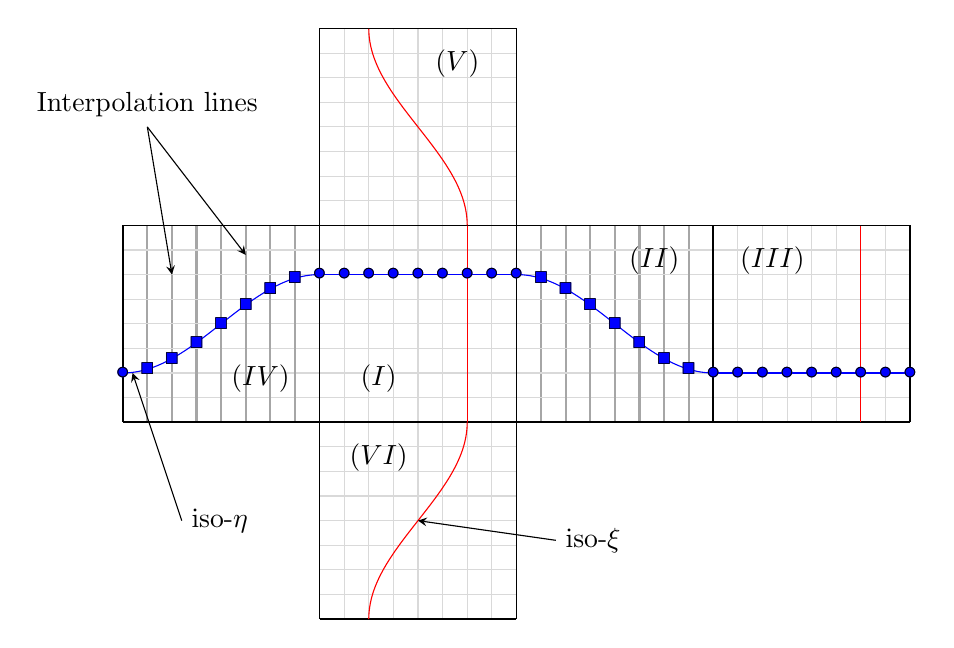
\begin{tikzpicture}[scale=2.5]
	\foreach \x in {1,...,7}
		{ \draw [color=gray!70, line width=0.8pt] (0.125*\x,1) -- (0.125*\x,2) ;
		\draw [color=gray!30] (0,1+0.125*\x) -- (1,1+0.125*\x) ;
		\draw [color=gray!30] (1+0.125*\x,1) -- (1+0.125*\x,2) ;
		\draw [color=gray!30] (1,1+0.125*\x) -- (2,1+0.125*\x) ;
		\draw [color=gray!70, line width=0.8pt] (2+0.125*\x,1) -- (2+0.125*\x,2) ;
		\draw [color=gray!30] (2,1+0.125*\x) -- (3,1+0.125*\x) ;
		\draw [color=gray!30] (3+0.125*\x,1) -- (3+0.125*\x,2) ;
		\draw [color=gray!30] (3,1+0.125*\x) -- (4,1+0.125*\x) ;
		\draw [color=gray!30] (1+0.125*\x,0) -- (1+0.125*\x,1) ;
		\draw [color=gray!30] (1,0.125*\x) -- (2,0.125*\x) ;
		\draw [color=gray!30] (1+0.125*\x,2) -- (1+0.125*\x,3) ;		
		\draw [color=gray!30] (1,2+0.125*\x) -- (2,2+0.125*\x) ;
		}
	

	\draw [line width=0.6pt] (1,3) -- (2,3) ; 
	\draw [line width=0.6pt] (0,2) -- (4,2) ; 	
	\draw [line width=0.6pt] (0,1) -- (4,1) ; 
	\draw [line width=0.6pt] (1,0) -- (2,0) ; 
	
	\draw [line width=0.6pt] (0,2) -- (0,1) ;
	\draw [line width=0.6pt] (1,3) -- (1,0) ;
	\draw [line width=0.6pt] (2,3) -- (2,0) ;
	\draw [line width=0.6pt] (3,2) -- (3,1) ;
	\draw [line width=0.6pt] (4,2) -- (4,1) ; 
	
	\draw (0.7,1.1) node[above]{$(IV)$} ; 
	\draw (1.3,1.1) node[above]{$(I)$} ; 
	\draw (2.7,1.7) node[above]{$(II)$} ;
	\draw (3.3,1.7) node[above]{$(III)$} ;  
	\draw (1.7,2.7) node[above]{$(V)$} ;  
	\draw (1.3,0.7) node[above]{$(VI)$} ; 
	
	\draw [samples=100,domain=0:1,color=blue] plot({\x},{1.5-(2*0.125)*cos(180*\x)});
	\draw [samples=100,domain=1:2,color=blue] plot({\x},{1.5+2*0.125});
	\draw [samples=100,domain=1:2,color=blue] plot({\x+1},{1.5-2*0.125*cos(180*\x)});
	\draw [samples=100,domain=3:4,color=blue] plot({\x},{1.5-2*0.125});
	\draw [>=stealth, <-] (0.05,1.25) -- (0.3,0.5) ;
	\draw  (0.3,0.5) node[right] {iso-$\eta$} ;
	
	\draw [samples=100,domain=0:1,color=red] plot({1.5-2*0.125*cos(180*\x)},{\x});
	\draw [samples=100,domain=1:2,color=red] plot({1.5+2*0.125},{\x});
	\draw [samples=100,domain=1:2,color=red] plot({1.5-2*0.125*cos(180*\x)},{\x+1});
	\draw [samples=100,domain=1:2,color=red] plot({4-+2*0.125},{\x});
	\draw [>=stealth, <-] (1.5,0.5) -- (2.2,0.4) ;
	\draw  (2.2,0.4) node[right] {iso-$\xi$} ;
	
	\draw  (0,1+2*0.125) node[color=blue] {$\bullet$} ;
	\draw (0,1+2*0.125) node {$\circ$} ;
	
	\foreach \k in {0,...,8}
		{\draw  (1+0.125*\k,1.5+2*0.125) node[color=blue] {$\bullet$} ;
	   	\draw (1+0.125*\k,1.5+2*0.125) node {$\circ$} ;
	   	\draw  (3+0.125*\k,1+2*0.125) node[color=blue] {$\bullet$} ;
	   	\draw (3+0.125*\k,1+2*0.125) node {$\circ$} ;
	   	}
	   	
	\foreach \x in {1,...,7}
		{\draw  ({0.125*\x},{1.5-2*0.125*cos(180*0.125*\x)}) node[color=blue] {\begin{tiny}$\blacksquare$\end{tiny}} ;
	   	\draw ({0.125*\x},{1.5-2*0.125*cos(180*0.125*\x)}) node {\begin{tiny}$\square$\end{tiny}} ;
	   	\draw  ({2+0.125*\x},{1.5-2*0.125*cos(180*0.125*\x+180)}) node[color=blue] {\begin{tiny}$\blacksquare$\end{tiny}} ;
	   	\draw  ({2+0.125*\x},{1.5-2*0.125*cos(180*0.125*\x+180)}) node {\begin{tiny}$\square$\end{tiny}} ;
	   	}
	   	
	\draw [>=stealth, <-] (0.25,1.75) -- (0.125,2.5) ;
	\draw [>=stealth, <-] (0.625,1.85) -- (0.125,2.5) ;
	\draw  (0.125,2.5) node[above] {Interpolation lines} ;
\end{tikzpicture}
\caption{Two typical great circles associated to
coordinate lines along the Cubed Sphere.
Compact differencing is carried out along each circle,
giving one-dimensional approximate derivatives.
Points marked with circles correspond to 
gridpoints where discrete values are located. In the contrary,
values must be interpolated at points marked with squares.}
\label{fig:patron cs}
\end{center}
\end{figure}
%%%%%%%%%%%%%%%%%%%%%%%%%%%%%%%%%%%%%%%%%%%%%%%%%%%%%%%%%%%%%%%%%%%%%%%
\begin{figure}[htbp]
\begin{center}
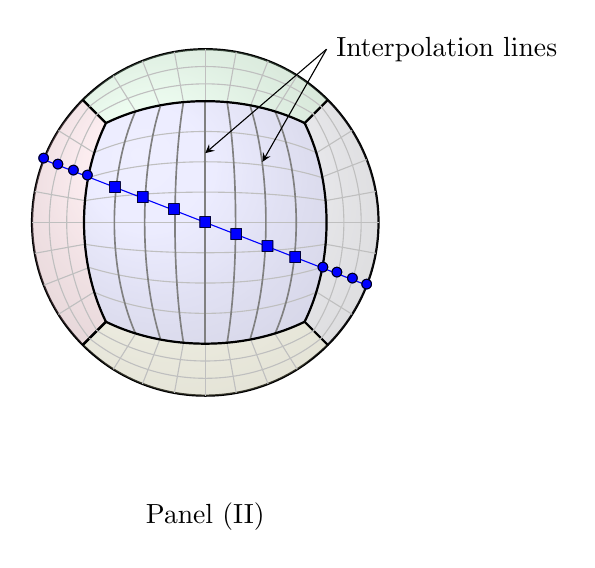
\begin{tikzpicture}[scale=2.2]
	\draw [line width=0.8pt] (0,0) circle (1cm);
    \shade[ball color=blue!10!white,opacity=0.20] (0,0) circle (1cm);	
	
	\filldraw[draw=black,fill=blue!30!white,opacity=0.20]
	plot [smooth,domain=-35:35] ({0.7*cos(\x)},{sin(\x)})
	-- plot [smooth,domain=55:125] ({cos(\x)},{0.7*sin(\x)})
	-- plot [smooth,domain=150:215] ({0.7*cos(\x)},{sin(\x)})
	-- plot [smooth,domain=240:300] ({cos(\x)},{0.7*sin(\x)})
	-- cycle;	
	\draw [samples=100,domain=48:132, color=gray!50] plot({cos(\x)},{0.35*sin(\x)});
	\draw [samples=100,domain=48:132, color=gray!50] plot({cos(\x)},{-.35*sin(\x)});
	\draw [samples=100,domain=46:134, color=gray!50] plot({cos(\x)},{0.175*sin(\x)});
	\draw [samples=100,domain=46:134, color=gray!50] plot({cos(\x)},{-.175*sin(\x)});
	\draw [samples=100,domain=50:130, color=gray!50] plot({cos(\x)},{0.525*sin(\x)});
	\draw [samples=100,domain=50:130, color=gray!50] plot({cos(\x)},{-.525*sin(\x)});
	\draw [samples=100,domain=45:135, color=gray!50] plot({cos(\x)},{0*sin(\x)});

	\draw [rotate=90, samples=100,domain=48:132, color=gray, line width=0.6pt] plot({cos(\x)},{0.35*sin(\x)});
	\draw [rotate=90, samples=100,domain=48:132, color=gray, line width=0.6pt] plot({cos(\x)},{-.35*sin(\x)});
	\draw [rotate=90, samples=100,domain=46:134, color=gray, line width=0.6pt] plot({cos(\x)},{0.175*sin(\x)});
	\draw [rotate=90, samples=100,domain=46:134, color=gray, line width=0.6pt] plot({cos(\x)},{-.175*sin(\x)});
	\draw [rotate=90, samples=100,domain=50:130, color=gray, line width=0.6pt] plot({cos(\x)},{0.525*sin(\x)});
	\draw [rotate=90, samples=100,domain=50:130, color=gray, line width=0.6pt] plot({cos(\x)},{-.525*sin(\x)});
	\draw [rotate=90, samples=100,domain=45:135, color=gray, line width=0.6pt] plot({cos(\x)},{0*sin(\x)});

	\filldraw[draw=black,fill=red!30!white,opacity=0.20]
	plot [smooth,domain=145:215] ({.7*cos(\x)},{sin(\x)})
	-- plot [smooth] (-.573,-.573) -- (-.707,-.707)
	-- plot [smooth,domain=215:145] ({cos(\x)},{sin(\x)})
	-- plot [smooth] (-.707,.707) -- (-.573,.573)
	-- cycle;	
	\draw [line width=0.8pt] (-.573,-.573) -- (-.707,-.707) ;
	\draw [line width=0.8pt] (-.573,.573) -- (-.707,.707) ;
	\draw [color=gray!50] (-.669,.260) -- (-.9321,.3622) ;
	\draw [color=gray!50] (-.669,-.260) -- (-.9321,-.3622) ;
	\draw [color=gray!50] (-.6946,.1259) -- (-.9840,.1783) ;
	\draw [color=gray!50] (-.6946,-.1259) -- (-.9840,-.1783) ;
	\draw [color=gray!50] (-.6427,.4022) -- (-.8477,.5305) ;
	\draw [color=gray!50] (-.6427,-.4022) -- (-.8477,-.5305) ;
	\draw [color=gray!50] (-.707,0) -- (-1,0) ;
	\draw [samples=100,domain=141:219, color=gray!50] plot({0.8*cos(\x)},{sin(\x)});
	\draw [samples=100,domain=138:222, color=gray!50] plot({0.9*cos(\x)},{sin(\x)});
	
	\filldraw[draw=black,fill=green!30!white,opacity=0.20]
	plot [smooth,domain=55:125] ({cos(\x)},{0.7*sin(\x)})
	-- plot [smooth] (-.573,.573) -- (-.707,.707)
	-- plot [smooth,domain=125:55] ({cos(\x)},{sin(\x)})
	-- plot [smooth] (.707,.707) -- (.573,.573)
	-- cycle;	
	\draw [line width=0.8pt] (-.573,.573) -- (-.707,.707) ;
	\draw [line width=0.8pt] (.707,.707) -- (.573,.573) ;
	\draw [rotate=-90,color=gray!50] (-.669,.260) -- (-.9321,.3622) ;
	\draw [rotate=-90,color=gray!50] (-.669,-.260) -- (-.9321,-.3622) ;
	\draw [rotate=-90,color=gray!50] (-.6946,.1259) -- (-.9840,.1783) ;
	\draw [rotate=-90,color=gray!50] (-.6946,-.1259) -- (-.9840,-.1783) ;
	\draw [rotate=-90,color=gray!50] (-.6427,.4022) -- (-.8477,.5305) ;
	\draw [rotate=-90,color=gray!50] (-.6427,-.4022) -- (-.8477,-.5305) ;
	\draw [rotate=-90,color=gray!50] (-.707,0) -- (-1,0) ;
	\draw [rotate=-90,samples=100,domain=141:219, color=gray!50] plot({0.8*cos(\x)},{sin(\x)});
	\draw [rotate=-90,samples=100,domain=138:222, color=gray!50] plot({0.9*cos(\x)},{sin(\x)});
	
	\filldraw[draw=black,fill=yellow!30!white,opacity=0.20]
	plot [smooth,domain=55:125] ({cos(\x)},{-.7*sin(\x)})
	-- plot [smooth] (-.573,-.573) -- (-.707,-.707)
	-- plot [smooth,domain=125:55] ({cos(\x)},{-sin(\x)})
	-- plot [smooth] (.707,-.707) -- (.573,-.573)
	-- cycle;	
	\draw [line width=0.8pt] (-.573,-.573) -- (-.707,-.707) ;
	\draw [line width=0.8pt] (.707,-.707) -- (.573,-.573) ;
	\draw [rotate=90,color=gray!50] (-.669,.260) -- (-.9321,.3622) ;
	\draw [rotate=90,color=gray!50] (-.669,-.260) -- (-.9321,-.3622) ;
	\draw [rotate=90,color=gray!50] (-.6946,.1259) -- (-.9840,.1783) ;
	\draw [rotate=90,color=gray!50] (-.6946,-.1259) -- (-.9840,-.1783) ;
	\draw [rotate=90,color=gray!50] (-.6427,.4022) -- (-.8477,.5305) ;
	\draw [rotate=90,color=gray!50] (-.6427,-.4022) -- (-.8477,-.5305) ;
	\draw [rotate=90,color=gray!50] (-.707,0) -- (-1,0) ;
	\draw [rotate=90,samples=100,domain=141:219, color=gray!50] plot({0.8*cos(\x)},{sin(\x)});
	\draw [rotate=90,samples=100,domain=138:222, color=gray!50] plot({0.9*cos(\x)},{sin(\x)});
	
	\draw [rotate=180,color=gray!50] (-.669,.260) -- (-.9321,.3622) ;
	\draw [rotate=180,color=gray!50] (-.669,-.260) -- (-.9321,-.3622) ;
	\draw [rotate=180,color=gray!50] (-.6946,.1259) -- (-.9840,.1783) ;
	\draw [rotate=180,color=gray!50] (-.6946,-.1259) -- (-.9840,-.1783) ;
	\draw [rotate=180,color=gray!50] (-.6427,.4022) -- (-.8477,.5305) ;
	\draw [rotate=180,color=gray!50] (-.6427,-.4022) -- (-.8477,-.5305) ;
	\draw [rotate=180,color=gray!50] (-.707,0) -- (-1,0) ;
	\draw [rotate=180,samples=100,domain=141:219, color=gray!50] plot({0.8*cos(\x)},{sin(\x)});
	\draw [rotate=180,samples=100,domain=138:222, color=gray!50] plot({0.9*cos(\x)},{sin(\x)});
	
	\draw [samples=100,domain=55:125, line width=0.8pt] plot({cos(\x)},{0.7*sin(\x)});
	\draw [samples=100,domain=55:125, line width=0.8pt] plot({cos(\x)},{-.7*sin(\x)});
	\draw [samples=100,domain=145:215, line width=0.8pt] plot({.7*cos(\x)},{sin(\x)}); 
	\draw [samples=100,domain=145:215, line width=0.8pt] plot({-.7*cos(\x)},{sin(\x)}); 
	
	\draw [color=blue] (-.9321,.3622) -- (.9321,-.3622) ;
	\draw  (-.9321,.3622) node[color=blue] {$\bullet$} ;
	\draw (-.9321,.3622) node {$\circ$} ;	
	\draw  (.9321,-.3622) node[color=blue] {$\bullet$} ;
	\draw (.9321,-.3622) node {$\circ$} ;
	\draw  (-.85,0.3886*.85) node[color=blue] {$\bullet$} ;
	\draw (-.85,0.3886*.85) node {$\circ$} ;	
	\draw (.85,-0.3886*.85) node[color=blue] {$\bullet$} ;
	\draw (.85,-0.3886*.85) node {$\circ$} ;	
	\draw  (-.76,0.3886*.76) node[color=blue] {$\bullet$} ;
	\draw (-.76,0.3886*.76) node {$\circ$} ;	
	\draw (.76,-0.3886*.76) node[color=blue] {$\bullet$} ;
	\draw (.76,-0.3886*.76) node {$\circ$} ;
	\draw  (-.68,0.3886*.68) node[color=blue] {$\bullet$} ;
	\draw (-.68,0.3886*.68) node {$\circ$} ;	
	\draw (.68,-0.3886*.68) node[color=blue] {$\bullet$} ;
	\draw (.68,-0.3886*.68) node {$\circ$} ;	
	\draw (-.52,0.3886*.52) node[color=blue] {\begin{tiny}$\blacksquare$ \end{tiny}} ;
	\draw (-.52,0.3886*.52) node {\begin{tiny}$\square$ \end{tiny}} ;
	\draw (.52,-0.3886*.52) node[color=blue] {\begin{tiny}$\blacksquare$ \end{tiny}} ;
	\draw (.52,-0.3886*.52) node {\begin{tiny}$\square$ \end{tiny}} ;
	\draw (-.36,0.3886*.36) node[color=blue] {\begin{tiny}$\blacksquare$ \end{tiny}} ;
	\draw (-.36,0.3886*.36) node {\begin{tiny}$\square$ \end{tiny}} ;
	\draw (.36,-0.3886*.36) node[color=blue] {\begin{tiny}$\blacksquare$ \end{tiny}} ;
	\draw (.36,-0.3886*.36) node {\begin{tiny}$\square$ \end{tiny}} ;
	\draw (-.18,0.3886*.18) node[color=blue] {\begin{tiny}$\blacksquare$ \end{tiny}} ;
	\draw (-.18,0.3886*.18) node {\begin{tiny}$\square$ \end{tiny}} ;
	\draw (.18,-0.3886*.18) node[color=blue] {\begin{tiny}$\blacksquare$ \end{tiny}} ;
	\draw (.18,-0.3886*.18) node {\begin{tiny}$\square$ \end{tiny}} ;
	\draw (0,0) node[color=blue] {\begin{tiny}$\blacksquare$ \end{tiny}} ;
	\draw (0,0) node {\begin{tiny}$\square$ \end{tiny}} ;
	
	\draw [>=stealth, <-] (.33,.35) -- (.7,1) ;
	\draw [>=stealth, <-] (0,.4) -- (.7,1) ;
	\draw  (0.7,1) node[right] {Interpolation lines} ;
	
	\draw  (0,-1.7) node {Panel (II)} ;

\end{tikzpicture}
\end{center}
\caption{Frontal view of panel (II) with the great circle in Fig. \ref{fig:patron cs}.
The points marked with squares are located on panel (II). They
do not belong to the grid (except several of them).
The value assigned to each point is deduced 
by a cubic spline interpolation along each vertical line.
This gives a 4th. order approximation at each of these points.
Doing the same on panel (IV), each point on the circle
carries a value, either exact or 4th. order accurate.
Applying the Hermitian derivative (\ref{eq:812.45}) at these points
gives an "almost" 4th. order derivative at 
points on panels (I) and (III). This procedure
is repeated along a set of great circles covering the Cubed Sphere.}
\label{fig: panel II_interp}
\end{figure}  
%%%%%%%%%%%%%%%%%%%%%%%%%%%%%%%%%%%%%%%%%%%%%%%%%%%%%%%%%%%%%%%%%
Consider for example in Fig. \ref{fig:patron cs}
the great circle marked with points. 
This circle crosses panels
$(I),(II),(III)$ and $(IV)$.
It coincides with coordinate lines in panels $(I)$ and $(III)$.
In panels $(II)$ and $(IV)$ it does not coincide with
coordinate lines.
%Consider now approximating the gradient $\nabla_T f$
%of some given function $f$. 
Based on the data on the Cubed Sphere $f^k_{i,j}$, 
one calculates Hermitian derivatives
along this circle. This is operated as follows.
First a suitable set of points $\bm_p$ is defined on this circle.
Second, values $f_p$ deduced from $f^k_{i,j}$ are assigned to these points. And third,
$\delta^H_\Delta f_{p}$ is calculated by (\ref{eq:812.45}).
The same calculation is performed in the $\eta-$ direction.
These calculations are repeated in the six panels.
At this point, we have at hand 
approximations $\delta^H_\xi f^k_{i,j}$ and
$\delta_\eta^H f^k_{i,j}$ at each point $\bss^k_{i,j}$ of the grid.
The approximate gradient
of the function $f$ is then deduced 
as follows. On the panel $k$, the local basis 
$(\bgg_\xi,\bgg_\eta)$ is
\beq
\label{eq:32.19}
\bgg_\xi(\mathbf{x})=\frac{\partial \mathbf{x}}{\partial \xi},\;\;\;
\bgg_\eta(\mathbf{x})=\frac{\partial \mathbf{x}}{\partial \eta}.
\eeq
Let $f(\bx)$ be a function defined on $\Bbb S_a$.
We denote by $f^\ast$ the restriction 
of $f$ to the grid points:
\beq
\label{eq:767.10}
(f^\ast)^k_{i,j}=f(\bs_{i,j}^k).
\eeq
The gradient of $f(\bx)$ is expressed in terms of the dual basis 
$(\bgg^\xi, \bgg^\eta)$ by
\begin{equation}
\label{eq:gradient}
\nabla_T f(\bx) = \dfrac{\partial f}{\partial \xi}(\bx) \mathbf{g}^{\xi}(\bx) 
+ \dfrac{\partial f}{\partial \eta}(\bx) \mathbf{g}^{\eta}(\bx).
\end{equation}
Using the two approximate values
\beq
\dfrac{\partial f}{\partial \xi}(\bss^k_{i,j}) \simeq \delta^H_\xi f^k_{i,j},\;\;\;
\dfrac{\partial f}{\partial \eta}(\bss^k_{i,j}) \simeq \delta^H_\eta f^k_{i,j},
\eeq
a natural approximate gradient $ \nabla_{T,\Delta} (f^\ast)_{i,j}^k $ 
is defined by (we note $\Delta=\Delta \xi=\Delta \eta$):
\begin{equation}
\label{eq:gradient_app}
\nabla_{T,\Delta} (f^\ast)_{i,j}^k 
=\delta^H_\xi (f^\ast)_{i,j}^k \mathbf{g}^{\xi}(\bss^k_{i,j}) 
+\delta^H_\eta (f^\ast)_{i,j}^k \mathbf{g}^{\eta}(\bss^k_{i,j}).
\end{equation}
The precise computational procedure proceeds in four steps
described in the Algorithm \ref{algo:41} hereafter. 
Consider again in Fig. \ref{fig:patron cs} the circle 
marked with points. This circle corresponds to some 
iso-$\eta$ line $\eta=\eta_0$ in panel (I). 
The main point is the extension of the $\xi$ coordinate
from the panel (I) to the full circle. This is detailed
in the steps 1 and 2 of Algorithm \ref{algo:41}.
As already said there is a calculation in the $\xi$ direction 
and a calculation in the $\eta$ direction
for the six panels, thus $12$ calculation in all. However, due
to the spherical symmetry, there is in fact only $6$ calculations
so that Algorithm \ref{algo:41} 
is applied to the $\xi$ and $\eta$ 
coordinate lines only in panels $(I)$, $(II)$ and $(V)$.
Overall, a set of $6 N$ great circles, covering the Cubed Sphere, are used. 
Finally, the values $\delta^H_{\xi}(f^\ast)^k_{i,j}$ and of 
$\delta^H_{\eta} (f^\ast)^k_{i,j}$ are obtained on the six panels 
and the approximation of the gradient is deduced
by (\ref{eq:gradient_app}). 
%%%%%%%%%%%%%%%%%%%%%%%%%%%%%%%%%%%%%%%%%%%%%%%%%%%%%%%%%%
\begin{center}
\begin{minipage}[]{12cm}
%\begin{minipage}[H]{12cm}
  \begin{algorithm}[H]
    \caption{: Hermitian derivative along the great 
circle in the $\xi-$ direction in Fig. \ref{fig:patron cs}.}\label{algo:41}
    \begin{algorithmic}[1]
     \State  {\sl Defining the grid on the great circle}. Consider 
a coordinate great circle based on a coordinate line in panel (I). We set
up as follows $4 N$ points on this circle (see Fig. \ref{fig:patron cs}) 
$\bm_p$, $p=0,\dots,4N$. The periodicity on this circle 
is expressed by $\bm_0=\bm_{4N}$.
\begin{enumerate}
	\item The first $N$ points $\bm_p = \bs^{(I)}_{p-N/2,j_0}$, $p=0, ..., N-1$ are located in panel (I). 
They belong to the Cubed Sphere and they carry 
values $f^{(I)}_{p-\frac{N}{2},j_0}$. They are represented by black circles in 
Fig. \ref{fig:patron cs}. 
	\item The next $N$ points $\bm_p$, $p=N...2N-1$ belong to panel (II).
They do not belong to the Cubed Sphere. Interpolated data of $f$ must be calculated 
at these points. They are represented by black squares 
in Fig. \ref{fig:patron cs}. These points play the role of auxiliary points. 
	\item The next $N$ points $\bm_p = s^{(III)}_{p-N/2,j_0}$, $p=2N, ..., 3N-1$ belong to panel (III). 
They belong to the Cubed Sphere and they carry 
values $f^{(III)}_{i,j_0}$. They are represented by black circles in 
Fig. \ref{fig:patron cs}. 
	\item The last $N$ points $\bm_p$, $p=3N...4N-1$ belong to panel (IV).
They do not belong to the Cubed Sphere. Interpolated data of $f$  must be calculated 
at these points. They are represented by black squares 
in Fig. \ref{fig:patron cs}. As in the panel (II), these points are auxiliary points.
\end{enumerate}

	\State {\sl Interpolation step}.
In this step data are interpolated from the Cubed-sphere to the points $\bm_p$:
\begin{enumerate}
\item In panels $(I)$ and $(III)$, the points
marked with black circles belong to the Cubed Sphere. 
Data $f^{(I)}_{p-N/2,j_0}$ are just copied
from the Cubed Sphere to the circle. There is no need of interpolation.
\item In panels $(II)$ and $(IV)$, a spline interpolation 
is performed as follows (see \cite{Croisille-10}).
The circle crosses vertical iso$-\xi$ lines. 
A cubic spline interpolation maps the data 
from the vertical iso$-\xi$ line to the points marked with black squares.
This gives a $4$th order interpolation for $f$ at these points.
\end{enumerate}

	\State {\sl Evaluating the Hermitian derivative on the circle}.
All the points $\bm_p$, $0 \leq p \leq 4 N$ now carry values.
The discrete derivative $\delta_{\xi}^H f_p$ is 
evaluated with (\ref{eq:812.45}).
This provides $4N$ (periodic) values called $\delta^H_\xi f_p$, $0 \leq p \leq 4N$.
The differentiation is operated with respect to
the equatorial angle. This angle coincides with the $\xi$-coordinate in the panel $(I)$ or $(III)$.

	\State {\sl Restricting the approximate derivative to coordinate lines}.
This step consists in retaining the components $\delta^H_\xi f_p$ 
located on panels 
$(I)$ and $(III)$ only. These components are stored. 
They correspond 
to indices $0 \leq p \leq N$, (panel (I)) and $2N \leq p \leq 3N$, (panel (III)).
The values of the derivatives in the panels $(II)$ and $(IV)$  
are also an outcome of the calculation. 
But they are useles since the points there do not belong to the Cubed Sphere. 
Therefore, they are not stored.

    \end{algorithmic}
    \end{algorithm}
\end{minipage}
\end{center}
%%%%%%%%%%%%%%%%%%%%%%%%%%%%%%%%%%%%%%%%%%%%%%%%%%%%%%%%%%%%%%%
\subsection{Approximation of differential operators}
\label{sec:op}
In Section \ref{sec:der_cs} we have shown how 
to approximate  the spherical gradient by (\ref{eq:gradient_app}).
Using the same principle, the divergence and the vorticity are approximated.
Consider a tangential vector field
$\bvv(\bx)$. The divergence and curl operators are
expressed in local coordinates as \cite{Simmonds}
\beq
\label{eq:95.13.1}
\left\{
\begin{array}{l}
\nabla_T \cdot \bvv= 
\partial_\xi \bvv \cdot  \bgg^\xi +\partial_\eta \bvv \cdot \bgg^\eta,
\;\;(a)\\
\nabla_T \times \bvv = 
\bgg^\xi \times \partial_\xi \bvv + \bgg^\eta \times \partial_\eta \bvv
\;\;(b).
\end{array}
\right.
\eeq
Consider the data $\bvv_{i,j}^{k}$ on the Cubed Sphere.
The discrete divergence and vorticity are defined by 
\beq
\left\{
\begin{array}{l}
\nabla_{T,\Delta} \cdot \bvv_{i,j}^{k}= 
\delta^H_\xi\bvv_{i,j}^{k} \cdot  (\bgg^\xi)_{i,j}^k 
+
\delta^H_\eta\bvv_{i,j}^{k} \cdot  (\bgg^\eta)_{i,j}^k,
\;\;(a), \\
\nabla_{T,\Delta} \times (\bvv)_{i,j}^k = 

(\bgg ^\xi)^k_{i,j}  \times \delta^H_\xi\bvv_{i,j}^{k}
+
(\bgg ^\eta)^k_{i,j}  \times \delta^H_\eta\bvv_{i,j}^{k}
\;\;(b).
\end{array}
\right.
\label{eq:div_rot}
\eeq
According to \eqref{eq:18.312}, we expect the discrete 
derivatives to be fourth order accurate. 
However, due to the interpolation of the data 
in Step 2 of Algorithm \ref{algo:41}, one may wonder 
if the accuracy could drop to $3$.
In fact, the value $f_p$ assigned to point $\bm_p$ on the circle
satisfies
\beq
\left\{
\begin{array}{l}
f_p = f(\bm_p) \mbox{ if } \bm \mbox { belongs to panels } (I) \mbox { or } (III).\\
f_p = f(\bm_p)+O(\Delta^4) \mbox{ if } \bm  \mbox { belongs to panels } (II) \mbox { or } (IV).
\end{array}
\right.
\eeq
Therefore it turns out that
\begin{equation}
(f_{p+1}-f_{p-1})/(2 \Delta \xi) = (f(\bm_{p+1})-f(\bm_{p-1}))/(2 \Delta \xi)
+O(\Delta ^3),
\end{equation}
which gives
\begin{equation}
\delta_{\xi}^H f_p = \partial_{\xi} f(\bm_p)
+O(\Delta ^3).
\end{equation}
As a consequence the approximations (\ref{eq:gradient_app}) and (\ref{eq:95.13.1})$_{a,b}$ are 
at least $O(\Delta ^3)$. In practice however, fourth order accuracy 
has been numerically observed so far.
\begin{remark}
There is some redundancy in the computation.
This is due to the fact that in Algorithm \ref{algo:41},
the Hermitian derivative in panel (II) and (IV) are
not retained. They just serve as auxiliary variables (or "ghost" values).0
\end{remark}
%%%%%%%%%%%%%%%%%%%%%%%%%%%%%%%%%%%%%%%%%%%%%%%%%%%%%%%%%%%%%%%%%%%%%%%%%%%%%%%%%%%
\subsection{Method of lines}
\label{sec:lines}
Consider for exemple the SWE system (\ref{eq:swe}).
It is rewritten as
\beq
\partial_t q(t,\bx)=J(q(t,\bx)),
\eeq
where the function $J(q)$ is
\begin{equation}
J(q) = 
\begin{bmatrix}
- \nabla_{T} \cdot \left( h^\star \mathbf{v}\right) \\
- \nabla_{T} \left( \dfrac{1}{2} |\mathbf{v}|^2 
+ g h \right) - \left( f + \zeta  \right) \mathbf{n}  \times \mathbf{v} 
\end{bmatrix}
.
\end{equation}
According to the method of lines, 
$J(q)$ is first approximated. Then
a time stepping scheme is applied.
The function $J(q)$ is approximated 
using the discrete operators 
\eqref{eq:gradient} and \eqref{eq:div_rot}$_{a,b}$. 
The semi discrete scheme is
\begin{equation}
\label{eq:81.10.8}
\dfrac{d \mathbf{q(t)}}{dt} = J_{\Delta} (\mathbf{q}(t)),
\end{equation}
where
$\mathbf{q}=[q^k_{i,j}]^T$ and ${-N/2 \leq i,j \leq N/2}$, $(I) \leq k 
\leq (VI)$. The discrete in sapce function $J_\Delta (\mathbf{q})$ is
%%%%%%%%%%%%%%%%%%%%%%%%%%%%%%%%%%%%%%%%%%%%%%%%%%%%%%%%%%
\begin{equation}
\label{eq:76.19}
J_{\Delta}(\mathbf{q}) = J_{\Delta}(h_{i,j}^k, \mathbf{v}_{i,j}^k) = 
\begin{bmatrix}
- \nabla_{T,\Delta} \cdot \left( h^{\star k}_{i,j} 
\mathbf{v}_{i,j}^k \right) \\
- \nabla_{T,\Delta} \left( \dfrac{1}{2} |\mathbf{v}_{i,j}^k|^2 
+ g h_{i,j}^k \right) - \left( f_{i,j}^k + \zeta_{i,j}^k \right) 
\mathbf{n}_{i,j}^k \times \mathbf{v}_{i,j}^k 
\end{bmatrix}
,
\end{equation}
where $\zeta_{i,j}^k = \left(\nabla_{T,\Delta} \times
 \mathbf{v}_{i,j}^k \right) \cdot \mathbf{n}_{i,j}^k$ is 
the semi discrete relative vorticity. 
Note that (\ref{eq:81.10.8}-\ref{eq:76.19}) is a non linear dynamical
system. It is expected to be fourth order accurate 
in $\Delta=\Delta \xi=\Delta \eta$.
There is no upwinding in the spatial approximation.
As a consequence, the accuracy of the
discrete equilibrium solutions are 4-th order as well.
In particular, the discrete equilibrium is not perturbed by the upwinding
of the flux function as in finite volume methods\footnote{
This perturbation requires the so-called well-balanced correction}. 
Refer to Section \ref{sec:4.2.3} for a numerical
example with the SW equations.
As we shall see in the numerical results,
there is no need for any additional numerical viscosity in space.
In fact, the intrinsic numerical viscosity of the RK4 scheme in Algorithm \ref{alg:RK4F}
presented in Section \ref{sec:13}
is sufficient for stability in most situations.
%%%%%%%%%%%%%%%%%%%%%%%%%%%%%%%%%%%%%%%%%%%%%%%%
\subsection{Time stepping scheme with filtering}
%%%%%%%%%%%%%%%%%%%%%%%%%%%%%%%%%%%%%%%%%%%%%%%%
\label{sec:13}
The time discretization is based on the classical Runge-Kutta order 4 
scheme to which a filtering operation is added at each time iteration. The time 
discretization is given by the
Algorithm \ref{alg:RK4F}.
%%%%%%%%%%%%%%%%%%%%%%%%%%%%%%%%%%%%%%%%%%%%%%%%%%%%%%%%%%%%%
\begin{center}
\begin{minipage}[H]{12cm}
  \begin{algorithm}[H]
%\label{algo:4}
    \caption{: Explicit Runge-Kutta Scheme of order 4 with filter}
\label{alg:RK4F}
    \begin{algorithmic}[1]
        \State $q^0 = q^{(0)}$ given
            \For{$n=0,1, \ldots$}
             \State  $K^{(1)} = J_{\Delta} \left( q^n \right)$,
             \State  $K^{(2)} = J_{\Delta} \left( q^n + \dfrac{\Delta t}{2} K^{(1)}\right)$,
             \State  $K^{(3)} = J_{\Delta} \left( q^n + \dfrac{\Delta t}{2} K^{(2)}\right)$,
             \State  $K^{(4)} = J_{\Delta} \left( q^n + \Delta t K^{(3)}\right)$,  
             \State  $q^{n+1} = \mathcal{F} \left( q^n  + \dfrac{\Delta t}{6} \left( K^{(1)} + 2 K^{(2)} + 2 K^{(3)} + K^{(4)} \right) \right)$.
            \EndFor
    \end{algorithmic}
    \end{algorithm}
\end{minipage}
\end{center}
In line 7 of Algorithm \ref{alg:RK4F}, $\mathcal{F}$ denotes the so-called {\sl filtering function}.
This filtering step eliminates the +1/-1 mode attached to the grid 
and improves the stability properties (see Section \ref{sec:annexes}).
On the Cubed-Sphere, we use a filter of the form
\begin{equation}
\mathcal{F} = \dfrac{1}{2} \left( \mathcal{F}_{\xi} \circ \mathcal{F}_{\eta} + \mathcal{F}_{\eta} \circ \mathcal{F}_{\xi} \right).
\end{equation}
The functions $\mathcal{F}_\xi$ and
$\mathcal{F}_\eta$ correspond to a $10$-th
order filter in the directions $\xi$ and $\eta$ respectively.
We refer to (\ref{eq:75.10.3}), (\ref{eq:11.101}) and 
the last line in Table \ref{tab:filter} 
for the $10$-th order
filter function which is used.
We let operate the filter function $\mathcal{F}_\xi$
along the great circles in a fashion similar to the 
operator $\delta^H_\xi$. The same 
steps than in Algorithm \ref{algo:41} are used.
As in Algorithm \ref{algo:41}, the data are completed 
by an interpolation procedure in the panels (II) and (IV). 
The difference between $\mathcal{F}$ and $\delta_\xi^H$ is that 
the operator $\mathcal{F}_\xi$ is explicit with a 
non compact stencil.

Several variants of compact formulas, of filter functions 
and of interpolation in the interpolation step of Algorithm \ref{algo:41} 
have been tested.
There is no evidence 
of better behaviour or accuracy with alternative choices.
Furthermore, the 10th order filter function in the last line 
of Table \ref{tab:filter}
is a good compromise between accuracy and stability.

%%%%%%%%%%%%%%%%%%%%%%%%%%%%%%%%%%%%%%%%%%%%%%%%%%%%%%%%%%%%%%%%%%%%%%%%%%%5
\section{Numerical results}
\label{sec:num}
In this section, we present numerical results obtained 
with our centered compact scheme.
We begin by showing results on the accuracy
of the discrete divergence and vorticity (\ref{eq:div_rot})
on particular exemples. 
Refer also to \cite{Croisille-10, Croisille-12}.

From Section \ref{sec:4.1} on, we consider 
the hyperbolic problems (\ref{eq:adv}), (\ref{eq:lswe}) and (\ref{eq:swe}).
In the three cases, the basic scheme relies on the same principle. 
First the equations are discretized in space.
This gives a system of the form
(\ref{eq:81.10.8}) by applying
the discrete space operators pointwise.
Second, the semi-discrete system is discretized in time
by the Algorithm \ref{alg:RK4F}.
 
Consider a non zero function $f(\bx)$ defined on $\Bbb S_a$ with restriction to
the grid $(f^\ast)^k_{i,j}=f(\bs^k_{i,j})$.
The error $e_p$, $p=1,2,\infty$ 
between $f^\ast $
and some approximant $\hat{f}^k_{i,j}$ is
defined by 
\begin{equation}
\label{eq:40.04}
e_p = \frac{\Vert(f^\ast)_{i,j}^{k} - \hat{f}^k_{i,j} \Vert_p}
{\Vert (f^\ast)_{i,j}^k \Vert_p}.
\end{equation}
In (\ref{eq:40.04}), the norm $\Vert . \Vert_p$ stands for
\beq
\Vert f^k_{i,j} \Vert_p= Q_N(\vert f \vert ^p)^{1/p},
\eeq
where $Q_N(f)$ denotes a quadrature rule
on the Cubed Sphere with parameter $N$. 
We have used the rule (20) in \cite{Portelenelle-Croisille},
which is of the form
\beq
\label{eq:87.10.1}
Q_N(f)= a^2\sum_{k=(I)}^{(VI)} \sum_{i,j=-N/2}^{N/2} \alpha_{i,j} (f^\ast)^k_{i,j},
\eeq
We refer to \cite {Portelenelle-Croisille}. for the definition 
of the weights $\alpha_{i,j}$.

Finally, note that the convergence analysis is performed by evaluating
the least squares fit for several grids.
%%%%%%%%%%%%%%%%%%%%%%%%%%%%%%%%%%%%%%%%%%%%
\subsection{Steady state in a spherical cap}
%%%%%%%%%%%%%%%%%%%%%%%%%%%%%%%%%%%%%%%%%%%%
This test was
suggested in \cite{BenArtzi-Falcovitz-LeFloch}.
Consider the scalar conservation law:
\beq
\label{eq:99.22}
\frac{\partial u}{\partial t}
+
\div_T \bF(x,u)=0.
\eeq
The sphere is $\Bbb S_a$ with $a=1$.
The tangential field $\bF(\bx,u)$ has the form
\beq
\bF(\bx,u)= 
\left[
\begin{array}{l}
x\\
y\\
z
\end{array}
\right]
\times
\left[
\begin{array}{l}
f_1(u)\\
f_2(u)\\
f_3(u)
\end{array}
\right].
\eeq
with
\beq
f_1(u)=f_2(u)=f_3(u)=\frac{1}{2}u^2.
\eeq
The function 
\beq
\label{eq:83.107}
u_0(x,y,z)=(x+y+z)/\sqrt{3}
\eeq 
is a time independent solution of (\ref{eq:99.22}).
Thus it can be compared at any time to 
the numerical solution. This enables
to assess the accuracy of the approximate divergence in a nonlinear context.
Fig. \ref{fig:57.21} reports at time $T=6$ the relative errors $e_p$, $p=1,2,\infty$
and the integral of $u$ on the sphere, which must remain constant
as time evolves. Fig. \ref{fig:57.22} reports the same quantities
but at time $T=600$.
In both cases, a coarse grid $32 \times 32 \times 6$,
is used with $\Delta t= \frac{0.96}{\pi} \Delta \xi$.
The growth remains bounded by small values in both cases, even at $T=600$.
Finally, Fig \ref{table:2.4.5} reports the convergence rate
at time $T=6$ using several grids. 
A convergence rate close to $4$ is observed in all norms.
%%%%%%%%%%%%%%%%%%%%%%%%%%%%%%%%%%%%%%%%%%%%%%%%%%%%%%%%%%%%%%%%%%%%
\begin{figure}[htbp]
\includegraphics[scale=0.4]{ref_7371265904_err.png}
\includegraphics[scale=0.4]{ref_7371265904_conservation.png}
\caption{Spherical cap test case: comparison between the time 
independent exact solution
$u_0(x,y,z)=(x+y+z)/\sqrt{3}$ and the approximate 
solution $u^k_{i,j}(t)$ for the conservation
law (\ref{eq:99.22}). 
Left panel: error history $e_p(t)
=
\Vert (u_0^\ast)_{i,j}^k-u^k_{i,j}(t)\Vert_p/ \Vert (u_0^\ast)_{i,j}^k \Vert_p$ 
with $p=1,2,\infty$ for $0 \leq t \leq T=6$. 
Right panel: conservation of the integral of $u(t,\bx)$ on the sphere.}
\label{fig:57.21}
\end{figure}
%%%%%%%%%%%%%%%%%%%%%%%%%%%%%%%%%%%%%%%%%%%%%%%%%%%%%%%%%%%%%%%%%%%%
\begin{figure}[htbp]
\includegraphics[scale=0.4]{ref_7371258652_err.png}
\includegraphics[scale=0.4]{ref_7371258652_conservation.png}
\caption{Same as Fig. \ref{fig:57.21} but on 
the time interval $0 \leq t \leq T=600$.}
\label{fig:57.22}
\end{figure}
%%%%%%%%%%%%%%%%%%%%%%%%%%%%%%%%%%%%%%%%%%%%%%%%%%%%%%%%%%%%%%%%%%%%%%
\begin{figure}[htbp]
\includegraphics[scale=0.5]{rate_test3.png}
\caption{Spherical cap test case: convergence for the steady state 
of (\ref{eq:99.22}). The error at time $T=6$ is reported. 
The convergence rate is close to $4$ in all norms.}
%%\label{table:2.4}
\label{table:2.4.5}
\end{figure}
%%%%%%%%%%%%%%%%%%%%%%%%%%%%%%%%%%%%%%%%%%%%%%%%%%%%%%%%%%%%%%%%%%%%%%%%%%%%%
\subsection{Accuracy of the approximate relative vorticity}
Consider a tangential vector field $\bvv$. 
The {\sl relative vorticity} is the scalar defined by
\begin{equation}
\vort_T (\mathbf{v}) = \left( \nabla_T \times \mathbf{v} \right) \cdot \mathbf{n}.
\end{equation}
A natural approximation is
\begin{equation}
\label{eq:33.10.3}
\vorth_{T,\Delta}(\mathbf{v}_{i,j}^{k}) = \left( \nabla_{T,\Delta} \times \mathbf{v}_{i,j}^{k} \right) \cdot \mathbf{n}(\mathbf{x}_{i,j}^{k}),
\end{equation}
where the operator $ \nabla_{T,\Delta} \times \mathbf{v}_{i,j}^{k} $  is defined in 
(\ref{eq:div_rot})$_{b}$.
The accuracy of (\ref{eq:33.10.3}) is assessed
with the two following tests, performed 
using functions defined on the spherical earth $\Bbb S_a$,
wit $a = 6.37122 \times 10^6\si{m}$ (earth radius).
%%%%%%%%%%%%%%%%%%%%%%%%%%%%%%%%%%%%%%%%%%%%%%%%%%%%%%%%%
\begin{enumerate}
\item
The first test consists in assessing numerically  the identity
\begin{equation}
\vort_T \left( \nabla_T h \right) = 0.
\label{eq:test3}
\end{equation}
We consider the particular case of the function $h(\bxx)$ defined
on $\Bbb S_a$ by
\beq
\label{eq:423.90}
h(\lambda, \theta) = \cos^5 (\theta) \sin(30 \lambda),
\eeq 
with $(\lambda, \theta)$ the longitudinal and latitudinal coordinates. 
The observed convergence rate in the norm $\Vert \,.\Vert_p/\vert \Bbb S_a \vert^{1/p}$
reported in Fig. \ref{fig:rate3} is close to $4$.
%%%%%%%%%%%%%%%%%%%%%%%%%%%%%%%%%%%%%%%%%%%%%%%%%%%%%%%%%%%%%%%%%%%%%%%%
\item
The second case represents a zonal wind with velocity
\begin{equation}
\mathbf{v}(\mathbf{x}) = \cos^{\alpha} (\theta) \mathbf{e}_{\lambda}(\mathbf{x}).
\label{eq:test1}
\end{equation}
The relative vorticity is 
\begin{equation}
\vort_T (\mathbf{v})(\mathbf{x}) = \dfrac{\alpha+1}{a} \cos^{\alpha-1} (\theta) \sin (\theta).
\end{equation}
Picking the parameter $\alpha \geq 2$ ensures
that the field and the relative vorticity
are regular near the poles.
We have choosen in our test $\alpha = 3$.
The relative error (\ref{eq:40.04}) is reported in 
Table \ref{tab:rate1} and 
in Fig. \ref{fig:rate1}. A sharp 4th. order
accuracy is observed in all norms.
%%%%%%%%%%%%%%%%%%%%%%%%%%%%%%%%%%%%%%%%%%%%%%%%%%%%%%%%%%%%%%%5
\begin{table}[htbp]
\begin{center}
\begin{tabular}{|c||c|c|c|}
\hline
\textbf{N}  & $\mathbf{e_1}$ & $\mathbf{e_2}$ & $\mathbf{e_{\infty}}$\\
\hline
\hline
$8$  & $2.9158 (-4)$ & $3.3039 (-4)$ & $6.7103 (-4)$ \\
$16$ & $1.7719 (-5)$ & $1.9906 (-5)$ & $4.0648 (-5)$ \\
$32$ & $1.1025 (-6)$ & $1.2416 (-6)$ & $2.5207 (-5)$ \\
$64$ & $6.9056 (-8)$ & $7.7821 (-8)$ & $1.6433 (-7)$ \\
$128$& $4.3244 (-9)$ & $4.8755 (-9)$ & $1.0822 (-8)$ \\
$256$& $2.7061(-10)$ & $3.0522(-10)$ & $6.9474(-10)$ \\
\hline 
\hline
\textbf{Rate}& $4.01$ & $4.01$ & $3.97$\\
\hline
\end{tabular}
\end{center}
\caption{Accuracy of the relative vorticity 
$\vort_{T,\Delta}(\bvv)$ 
for the tangential field 
$\mathbf{v}(\mathbf{x}) = \cos^{\alpha} (\theta) \mathbf{e}_{\lambda}(\mathbf{x})$.
The relative error $e_p$ given in \eqref{eq:40.04} with $p=1$, $2$, $\infty$. 
A sharp $4$-th order accuracy is observed in all norms.}
\label{tab:rate1}
\end{table} 
%%%%%%%%%%%%%%%%%%%%%%%%%%%%%%%%%%%%%%%%%%%%%%%%%%%%%%%%%%%%%%%%%%%%%%%
\begin{figure}
 \begin{minipage}[b]{.46\linewidth}
  \includegraphics[height=4.9cm]{rate_vort3.png}
  \caption{Accuracy of the identity $\vort_T \left( \nabla_T h \right) = 0.$,
with test case (\ref{eq:test3}) and the function 
$h(\lambda, \theta) = \cos^5 (\theta) \sin(30 \lambda)$.
The errors $\Vert . \Vert_p$ (normalized with $\vert \Bbb S_a\vert^{1/p}$) 
are reported with 
$p=1,2$ and $\infty$. The grid $N=8$ is too coarse to represent the function $h$.
 \label{fig:rate3}}
 \end{minipage}\hfill
 \begin{minipage}[b]{.46\linewidth}
  \includegraphics[height=5.cm]{rate_vort1.png}
  \caption{Accuracy 
of the relative vorticity (\ref{eq:33.10.3}) for the tangential field 
$\mathbf{v}(\mathbf{x}) = \cos^{3} (\theta) \mathbf{e}_{\lambda}(\mathbf{x})$.
Convergence rate of the approximate relative vorticity of \eqref{eq:test1}
 for $e_p$ with $p=1,2$ and $\infty$ with the same grid parameter 
than in Fig. \ref{fig:rate3}.\label{fig:rate1}}
 \end{minipage}
\end{figure}
%%%%%%%%%%%%%%%%%%%%%%%%%%%%%%%%%%%%%%%%%%%%%%%%%%%%%%%%%%%%%%%%%%%%%%
% \item
% In the third case, we consider for 
% $\bx=[x,y,z]^T \in \Bbb S^2_a$, the tangential vector 
% field defined by
% \begin{equation}
% \mathbf{v}(\mathbf{x}) = \mathbf{n}(\mathbf{x}) \times
% \begin{bmatrix}
% \exp (y/a) \\ \exp (x/a) \\ \exp (z/a)
% \end{bmatrix}.
% \label{eq:test2}
% \end{equation}
% The exact relative vorticity is
% \begin{equation}
% \vort_T(\bvv)(\bx) 
% = \dfrac{1}{a} \mathbf{n}(\mathbf{x}) \times \begin{bmatrix}
% -\left( 2 + \frac{z}{a} \right) \exp \left( z/a \right) \\[10pt]
% -\left( 2 + \frac{x}{a} \right) \exp \left( x/a \right) \\[10pt]
% -\left( 2 + \frac{y}{a} \right) \exp \left( y/a \right) 
% \end{bmatrix}.
% \end{equation}
% The results are similar to case 2 (not shown).
\end{enumerate}

%%%%%%%%%%%%%%%%%%%%%%%%%%%%%%%%%%%%%%%%%%%%%%%%%%%%%%%%%%%%%%%%
\subsection{Deformational flow with vortices}
\label{sec:4.1}
We consider the convection equation
\begin{equation}
\label{eq:adv-2}
\dfrac{\partial h}{\partial t}  (t,\mathbf{x})+ \mathbf{c}(t,\mathbf{x}) 
\cdot \nabla_T h(t,\mathbf{x})=0
\end{equation}
The velocity $\mathbf{c}(t,\mathbf{x})$ is prescribed 
to let evolve the initial condition 
with two constant states on a half sphere 
%%into a rollup structure, see Fig. \ref{fig:}.
into a rollup structure.
This structure consists of two vortices localised at two diametraly 
opposite points $C$ and $C'$. 
As time evolves, filaments
spiral around the two vortex centers. This behaviour
is well known in point vortex flows.
This test was introduced in \cite{Nair-Machenhauer, Nair-Jablonowski}
as a sequel of the solid body test case (test 1) in 
\cite{Williamson-Drake-Hack-Jakob-Swarztrauber}.
Here the analytical solution is available by the characteristics method.
This case is challenging
to evaluate the spatial accuracy, since
the filaments go below the resolution of the grid at some
time. The time stepping accuracy is also evaluated.
Two variants were introduced in
\cite{Nair-Machenhauer,Nair-Jablonowski}.
In the first variant, the velocity $\bc$ is
time independent. It is given 
in the coordinate system $(\lambda', \theta')$ 
attached to the axis $(C C^\prime)$
by
\begin{equation}
\label{eq:34.981}
\bc(\bx)=a c_{\lambda'}(\bx) \be_{\lambda'}(\bx),
\end{equation}
where
\begin{equation}
c_{\lambda'}=\cos(\theta') \omega_r(\theta'),\;\;
   \omega_r ( \theta') = \left\{ 
   \begin{array}{ll}
      V(\theta')/( a \rho(\theta') ) & \text{ if } \rho \neq 0, \\
      0 & \text{ if } \rho =0.
   \end{array}
   \right.
\label{vitesse_angulaire}
\end{equation}
and 
\begin{equation}
\left\{
\begin{array}{l}
\rho(\theta')=\rho_0 \cos(\theta'),\\
V(\theta') = u_0 \dfrac{3 \sqrt{3} }{2} \sech^2 ( \rho(\theta') ) \tanh ( \rho(\theta') ).
\end{array}
\right.
\end{equation}
with parameters $T>0$, $\rho_0>0 $ and $ u_0 = 2 \pi a / T$. 
The solution $ h(t,\bx)$ is given in coordinates $(\lambda',\theta')$ 
by
\begin{equation}
h(t,\lambda',\theta')=
1 - \tanh \Big( \dfrac{\rho(\theta')}{\gamma} \sin ( \lambda' 
- \omega_r(\theta') t ) \Big),
\label{NM_exacte}
\end{equation}
The values 
$\rho_0 = 3$, $ \gamma = 5$, $T=12$ days (in seconds)
and earth radius $a = 6.37122 \times 10^6\si{m}$.
Fig. \ref{fig:57.2} reports 
the error history when the point $C$ 
is at $(\lambda_C, \theta_C) = (\pi/4, \pi/4)$. 
It corresponds 
to a location of the vortices at the intersection
of three panels. This test permits to assess 
the accuracy of the approximate gradient with Algorithm \ref{algo:41}.
The grid is fixed $36 \times 36 \times 6$. It is
a coarse grid, with equatorial resolution $\Delta \lambda = 2.5 \deg$. 
Two time steps were used 
to reach $T=12$ days. In both cases, the scheme
was found stable with a smoothly growing error.
When performing 2880 iterations, the error is dominated by the spatial approximation.
The observed error levels are comparable to the ones
obtained  with the Discontinuous Galerkin method in \cite{Nair-Jablonowski}.
With 288 iterations, space and time errors are observed simultaneously.
and the error level is slightly better 
in that case.
Fig. \ref{table:2.4} reports the convergence rate 
in the norms $p=1$, $p=2$ and $p=\infty$ with 205 iterations. The error convergence
is of order greater than $4$, which is better than expected.
%%%%%%%%%%%%%%%%%%%%%%%%%%%%%%%%%%%%%%%%%%%%%%%%%%%%%%%%%%%%%%%%%%%%%%%%%%%%%%
\begin{figure}[htbp]
\includegraphics[scale=0.3]{ref_7367656360_normerreur_test_1.png}
\includegraphics[scale=0.3]{ref_7367656531_normerreur_test_1.png}
%\includegraphics[scale=0.4]{ref_7367665245_normerreur_test_1.png}
\caption{Deformational test case, time independent velocity,
\cite{Nair-Machenhauer, Nair-Jablonowski}. 
The axis $(CC^\prime)$ is such that 
$(\lambda_C,  \theta_C) = (\pi / 4, \pi / 4)$.
Grid $36 \times 36\times 6$. 
Left panel: error history with 2880 iterations. 
Right panel: error history with 288 iterations. 
\label{fig:57.2}
}
\end{figure}
%%%%%%%%%%%%%%%%%%%%%%%%%%%%%%%%%%%%%%%%%%%%%%%%%%%%%%%%%%%%%%%%%%%%%%%%%
\begin{figure}[htbp]
\includegraphics[scale=0.5]{rate_NMpi4.png}
\caption{Deformational test case, 
time independent velocity (\ref{eq:34.981}).
% \cite{Nair-Machenhauer, Nair-Jablonowski}. 
Convergence analysis at day $12$. $(\lambda_C, \theta_C) = (\pi/4,\pi/4)$. 
With the grid $N \times N \times 6$, the time step is such that
$ \frac{2 \pi u_0 \Delta t}{N}=0.9$. The accuracy is close to $5$.}
\label{table:2.4}
\end{figure}
%%%%%%%%%%%%%%%%%%%%%%%%%%%%%%%%%%%%%%%%%%%%%%%%%%%%%%%%%%%%%%%%%%%%%%%%%

The second variant \cite{Nair-Jablonowski} 
consists in superposing to the preceding velocity a 
solid body rotation at constant speed.
As a result, the rollup behaviour of the two antipodal vortices
is now superposed to the traveling wave effect 
at constant speed. 
This makes the test more difficult 
for large time than the previous one. The velocity  $\mathbf{c}(t,\mathbf{x})$ in \eqref{eq:adv-2} 
is $\mathbf{c}(t,\bx)
=
\mathbf{c}_s(\bx) +\mathbf{c}_r(t,\bx)$
where 
$\mathbf{c}_r$ is the "static" velocity in (\ref{eq:34.981}) and
$\mathbf{c}_s$ is the solid rotation velocity defined by
\begin{equation}
\label{eq:34.989}
\bc_s(\bx)=c_{\lambda,s}(\bx) \be_{\lambda}(\bx)+c_{\theta,s}(\bx) \be_{\theta}(\bx)
\end{equation}
with
\begin{equation}
\left\{
\begin{array}{l}
c_{\lambda, s} = u_0 (\cos \theta \cos \alpha + \sin \theta \cos \lambda \sin \alpha),\\
c_{\theta, s} = -u_0 \sin \lambda \sin \alpha.
\end{array}
\right.
%\label{vitesse_theta_bump}
\end{equation}
The parameters are the rotation angle $\alpha$ and 
$u_0 = 2 \pi a / (12 \rm{days})$.
In (\ref{NM_exacte})
the point $C$ is now moving
along solid body rotation. 
Its coordinates $(\lambda^\prime_C(t),\theta^\prime_C(t))$ 
are 
\begin{equation}
(\lambda^\prime_C(t), \theta^\prime_C(t)) = (\lambda_0 + \omega_s t, \theta_0),
\end{equation}
where $(\lambda_0, \theta_0) = (3 \pi /2, 0)$ is the initial 
position of the vortex.
The "static" velocity $\bc_s(t,\bx)$ is 
\beq
\label{eq:546.93}
\bc_r(t,\bx)=c_{\lambda,r}(t,\bx) \be_{\lambda}(\bx)+c_{\theta,r}(\bx) \be_{\theta}(\bx)
\eeq
with
\begin{equation}
\left\{
\begin{array}{l}
c_{\lambda, r}(t) = a \omega_r \Big[ \sin \theta_C(t) \cos \theta - 
\cos \theta_C(t) \cos ( \lambda - \lambda_C(t) ) \sin \theta \Big],\\
c_{\theta, r}(t) = - a \omega_r \cos \theta_C(t) 
\sin ( \lambda - \lambda_C(t) ).
\end{array}
\right.
%\label{vitesse_theta_bump}
\end{equation}
where $\omega_r = u_0/a=2 \pi / (12 \rm{days}) $ 
and $( \lambda_C(t), \theta_C(t))$
is the coordinates of the moving point $C$.

At $T=12$ days, the 
error level is comparable to the Discontinous Galerkin approximation 
in \cite{Nair-Jablonowski}. 
We also compare the results 
using two upwind finite volume schemes 
with high order reconstruction \cite{Katta-Nair-Kumar}.
These two schemes 
are referred to as WENO5 and KL4 respectively.
We have used the parameter $\alpha=\pi/4$. The grid is  $80 \times 80 \times 6$ 
and $750$ times iterations are performed (at $T=12$ days). 
Typical results reported  
\cite{Katta-Nair-Kumar}
with the WENO5 scheme give errors 
of $e_1=0.0021$, $e_2=0.0042$ and 
$e_{\infty} = 0.0191$. Using the KL4 scheme, errors are 
reported as $e_1=0.0021$, $e_2=0.0043$ and $e_{\infty}=0.0194$. 
With the present scheme, using the parameters above, the observed errors 
are $e_1=1.67(-4)$, $e_2=7.23(-4)$ and $e_{\infty}=5.75(-3)$
which is slightly better.
In Fig. \ref{coupe-NJ-1} a slice of the vortex after $12$ days
is represented with resolution $N=30$ and $N=60$, respectively. 
With a resolution $N=60$, an excellent match 
with the exact solution is observed. Table \ref{table:2} reports
fourth order at final time.

Finally, we report in Fig. \ref{fig:43.98}
the relative error history
during a larger time of $T=24$ days.
This permits to observe the potential
of the scheme at a time where a lack of accuracy is
expected. 
We have used first a coarse grid $40 \times 40 \times 6$ with 457 time iterations
and second a fine grid $80 \times 80 \times 6$ with
914 time iterations. 
With the coarse grid, 
the error level after $24$ days is $15.93\%$ in the maximum norm
and $3.67 \%$ in the $L^2$ norms. 
With the fine grid, the errors is below $9.63\%$ 
for the maximum norm
and $1.69 \%$ with the $L^2$ norms.
%%%%%%%%%%%%%%%%%%%%%%%%%%%%%%%%%%%%%%%%%%%%%%%%%%%%%%%%%%%%%%%%%%%%%%%
\begin{figure}[htbp]
\includegraphics[scale=0.25]{coupe.png}
\caption{Deformational test case, time dependent velocity (\ref{eq:546.93}).
%\cite{Nair-Jablonowski}. 
Slice 
of the vortex after $12$ days: the value of $h$ in (\ref{eq:adv-2}) is
displayed in function of the longitude angle (in radians). Solid line: exact solution. Circles:
approximate solution with the grid 
$30 \times 30 \times6$. Crosses: approximate solution with the grid 
$60 \times 60 \times 6$.}
\label{coupe-NJ-1}
\end{figure}
%%%%%%%%%%%%%%%%%%%%%%%%%%%%%%%%%%%%%%%%%%%%%%%%%%%%%%%%%%%%%%%%%%%%%%%%%%%%%%
\begin{figure}[htbp]
\includegraphics[scale=0.5]{rate_NJ.png}
\caption{Deformational test case, time dependent velocity (\ref{eq:546.93}).
%\cite{Nair-Jablonowski}.
The time step is given by 
$2 \pi u_0 \Delta t/N = 0.7$ with $u_0= 2 \pi a /12\rm{12 days}$,
the earth radius $a$ 
and $\alpha = \pi /4$.
Convergence slope at final time in the three norms $e_p$, $p=1,2,\infty$.
}
\label{table:2}
\end{figure}
%%%%%%%%%%%%%%%%%%%%%%%%%%%%%%%%%%%%%%%%%%%%%%%%%%%%%%%%%%%%%%%%%%%%%%%%%%%%
 \begin{figure}[htbp]
% \includegraphics[scale=0.4]{ref_7367657290_normerreur_test_2.png}
 \includegraphics[scale=0.4]{ref_7371125384_normerreur_test_2.png}
 \includegraphics[scale=0.4]{ref_7371124908_normerreur_test_2.png}
 \caption{Deformational test case, time independent velocity
\cite{Nair-Jablonowski}. 
The angle parameter is $\alpha = \pi/4$.
The error history of the relative error is reported 
for $24$ days. Left panel: grid $40\times40\times6$ and $457$ time iterations. 
The relative error levels are after $24$ days: 
$L^1$ norm: $1.36 \%$,
$L^2$ norm: $3.67 \%$,
$L^\infty$ norm: $15.93 \%$,
  Right panel: grid resolution $80\times 80 \times6$ and $914$ time iterations.
The relative error levels are after $24$ days: 
$L^1$ norm: $0.45 \%$,
$L^2$ norm: $1.69 \%$,
$L^\infty$ norm: $9.63 \%$,
 }
 \label{fig:43.98}
%% erreur_cfl=0.05a}
 \end{figure}
%%%%%%%%%%%%%%%%%%%%%%%%%%%%%%%%%%%%%%%%%%%%%%%%%%%%%%%%%%%%%%%%%%%%%%
\subsection{Linearized shallow water equation}
\label{sec:4.2}
We consider the shallow water equation \eqref{eq:lswe}
linearized around an atmosphere at rest.
We consider two cases designed 
using hand manufactured solutions. The source terms 
$S_\eta$ and $S_\bvv$ are adjusted to these solutions.
The numerical scheme uses the approximation 
(\ref{eq:gradient} - \ref{eq:div_rot})
with the filtered RK4 scheme (Algorithm \ref{alg:RK4F}).
As before, the approximation in space is centered.

The first test case  serves to assess the accuracy of the 
approximate gradient and divergence (\ref{eq:gradient}) and (\ref{eq:div_rot}) when
used in the LSWE system (\ref{eq:lswe}). 
Consider the two exponentially in time damped functions
\begin{equation}
\label{eq:90.92}
\left\lbrace
\begin{array}{rcl}
\tilde{\eta}(t,\mathbf{x}) & = & \varphi(\theta) e^{-\sigma t},\\[10pt]
\tilde{\mathbf{v}} (t,\mathbf{x}) & = & \dfrac{\sqrt{g H}}{10} \varphi(\theta) e^{-\sigma t}\mathbf{e}_\lambda(\mathbf{x}).
\end{array}
\right.
\end{equation}
with
\begin{equation}
\label{eq:fct_galewsky}
\varphi(\theta) = 
\left\lbrace
\begin{array}{ll}
0 & \text{ if } \theta \leq \theta_0, [10pt]\\
\dfrac{1}{e_n} \exp \left[ \dfrac{1}{(\theta - \theta_0)(\theta - \theta_1)} \right] 
& \text{ if } \theta_0 \leq \theta \leq \theta_1, [10pt]\\
0 & \text{ if } \theta_1 \leq \theta.
\end{array}
\right.
\end{equation}
The normalization constant $e_n=\exp \left[ \dfrac{-4}{(\theta_0 - \theta_1)^2} \right]$
gives $\varphi(\theta_0)=\varphi(\theta_1)=1$.

We have picked $\sigma = 10^{-5}$, $\theta_0=-\pi/3$, $\theta_1=\pi/3$. 
The system to be solved is (\ref{eq:lswe}) where the source terms 
$S_{\eta}$ and $S_{\mathbf{v}}$ 
are defined 
such that $(\tilde \eta(t,\mathbf{x}),\tilde{\mathbf{v}}(t,\mathbf{x}))^T$
is solution. 
In Fig. \ref{table:4}, left panel, 
the least squares slope is reported 
using three grids.
%%%%%%%%%%%%%%%%%%%%%%%%%%%%%%%%%%%%%%%%%%%%%%%%%%%%%%%%%%%%%%%%
\begin{figure}[htbp]
\includegraphics[scale=.5]{rate_lswe_exp.png}
\includegraphics[scale=.5]{rate_lswe_stat.png}
\caption{Convergence of the compact scheme
in the case of the LSWE equations (\ref{eq:lswe}). 
Left panel: the Hermitian scheme applied to the exponential decaying solution (\ref{eq:90.92}) 
of the LSWE. The source term $S_\eta$ and $S_\bvv$ are adjusted to 
the decaying solution (\ref{eq:90.92}).  The final time is 1.5 hour and $H=10^5$ meters.
Right panel: time independent zonal solution (\ref{eq:78.123}) and (\ref{eq:78.125}) 
of the LSWE system.
The slope is very close in the two cases. The observed error level
is better in the time independent case.
}
\label{table:4}
\end{figure}
%%%%%%%%%%%%%%%%%%%%%%%%%%%%%%%%%%%%%%%%%%%%%%%%%%%%%%%%%%%%%%%%%%%

The second case is a time independent zonal solution.
To a parameter function $\varphi(\theta)$ given by \eqref{eq:fct_galewsky} 
corresponds the velocity $\mathbf{v}(\mathbf{x})$ defined by
\begin{equation}
\label{eq:78.123}
\mathbf{v}(\mathbf{x})=u_0 \varphi(\theta) \mathbf{e}_\lambda(\mathbf{\theta}).
\end{equation}
Integrating the momentum equation (\ref{eq:lswe})$_2$ 
gives
\begin{equation}
\label{eq:78.125}
\eta(\mathbf{x})=\eta_{eq}-\frac{a \cdot u_0}{g}\int_0^\theta f(s) \varphi(s) ds.
\end{equation}
The functions (\ref{eq:78.123}) and (\ref{eq:78.125}) are
a zonal divergence free solution
of (LSWE).
This test case serves to assess the accuracy of the approximation in space. 
In particular, the accuracy of the zero divergence 
preserving for large time.
The numerical results are reported in the right panel in Fig. \ref{table:4}.
%%%%%%%%%%%%%%%%%%%%%%%%%%%%%%%%%%%%%%%%%%%%%%%%%%%%%%%%%%%%%%%%%%%%
\subsection{Shallow Water equations}
Numerical results are displayed on
four standard test cases involving the (SW) system 
\eqref{eq:swe}.
As in Sections \ref{sec:4.1} and \ref{sec:4.2} we use the scheme 
(\ref{eq:81.10.8}). The differential operators
gradient, divergence and vorticity are discretized 
directly without any upwinding by
(\ref{eq:gradient}-\ref{eq:div_rot}). The time scheme
is given in Algorithm \ref{alg:RK4F}. 
First, the cases 2, 5 and 6
from the standard suite \cite{Williamson-Drake-Hack-Jakob-Swarztrauber}
are considered.
They are refered to as the geostrophic steady-state flow, 
the isolated mountain case and the Rossby-Haurwitz case.
The fourth case is the barotropic instability 
case of Galewsky {\sl et al.} \cite{Galewsky-Scott-Polvani}.
In all cases the results are compared 
to the literature.
As we shall see, the compact scheme behaves very well
in all cases.
The conservation properties
of the scheme are also numerically analyzed.
The constants are 
$a = 6.37122 \times 10^6\si{m}$ (earth radius),
$\Omega = 7.292 \times 10^{-5} \si{s^{-1}}$ (earth angular velocity),
and $g = 9.80616 \si{m . s^{-2}}$ (gravity constant).
The Coriolis force is $f(\bx)=2 \Omega \sin \theta$.

The following averaged values are preserved at the continuous level.
\begin{itemize}
\item mass : $I_1=\gint_{\mathbb{S}_a^2} h^{\star}d\mathbf{s}$,

\item energy : $I_2 = \gint_{\mathbb{S}_a^2} \frac{1}{2} h^{\star} \mathbf{v}^2 
+ \frac{1}{2}g \left( h^2 - h_s^2 \right) d\mathbf{s}$,

\item potential enstrophy : $I_{3}=\gint_{\mathbb{S}_a^2} 
\dfrac{\left( \zeta + f \right)^2}{2 h^{\star}} d\mathbf{s}$ with $\zeta$ the 
relative vorticity,

\item
divergence :
$I_4 = \frac{1}{\vert \Bbb S_a \vert}
\gint_{\mathbb{S}_a^2}  \nabla_T \cdot \mathbf{v} d\mathbf{s}$,

\item
relative vorticity:
 $I_5 = \frac{1}{\vert \Bbb S_a \vert}
\gint_{\mathbb{S}_a^2}  \left( \nabla_T \times \mathbf{v}  \right) \cdot \mathbf{n} 
d\mathbf{s}$.
\end{itemize}
%According to \cite{Williamson-Drake-Hack-Jakob-Swarztrauber},
The numerical error  
for $I_1$, $I_2$ and $I_3$ is reported using the relative (algebraic) value 
\begin{equation}
\label{eq:relative_error_cons}
\dfrac{ I_p(t)-I_p(0)}{ I_p(0) }, p=1,2,3.
\end{equation}
In the two last cases, the value of $I_4$ and $I_5$ is reported.
In all cases, the numerical integrals are calculated by (\ref{eq:87.10.1}).
%%%%%%%%%%%%%%%%%%%%%%%%%%%%%%%%%%%%%%%%%%%%%%%%%%%%%%%%%%%%%%%%%
\subsubsection{Time-independent geostrophic flow}
\label{sec:4.2.3}
The test case 2 in \cite{Williamson-Drake-Hack-Jakob-Swarztrauber}
consists in assessing the accuracy in space
of the scheme for a 
zonal time independent solution of (\ref{eq:swe}).
The angle $\alpha$ is a parameter representing
the angle of an axis with the $Oz$ direction.
This parameter serves to observe the influence
of the position of the grid with respect to
the zonal equilibrium solution. 
In our case, it permits to evaluate 
how the Cubed Sphere operates with
an oblique orientation. 
The Coriolis force is expressed as
\begin{equation}
f(\bx)=2 \Omega \left( - \cos \lambda \cos \theta \sin \alpha + \sin \theta \cos \alpha \right).
\end{equation}
The exact solution is $(h,\bvv)$, with
$\mathbf{v} = u \mathbf{e}_{\lambda} + v \mathbf{e}_{\theta}$:
\begin{equation}
\left\lbrace
\begin{array}{rcl}
h & = & h_0- \dfrac{1}{g} \left( a \Omega u_0 + \dfrac{u_0^2}{2} \right) 
\left( -\cos \lambda \cos \theta \sin \alpha + \sin \theta \cos \alpha \right)^2,\\[10 pt]
u & = & u_0 \left( \cos \theta \cos \alpha + \cos \lambda \sin \theta \sin \alpha \right),\\[10 pt]
v & = & -u_0 \sin \lambda \sin \alpha.
\end{array}
\label{eq:W2 velocity}
\right.
\end{equation}
The constants $g h_0$ is
$gh_0 = 2.94 \times 10^4 \si{m^2.s^2}$ and
$u_0 =  2 \pi a / (12 \text{days})$ ( in $ \si{m.s^{-1}}$).
Fig. \ref{fig:W2 err alpha=pi/4}
shows the history of the relative error on $h$
in the case $\alpha=\pi/4$.
Error growths are monotonic and very slow.
Fig. \ref{tab:W2 error order} reports 
the convergence slope for $h$. In both cases ($\alpha=0$ and $\alpha=45$),
a sharp 4-th order accuracy is obtained.
The error $e_\infty$ at day $5$ is close to $2.78\;10^{-6}$ to be compared
with $5.86\; 10^{-6}$ in \cite{Chen-Xiao} (Table 5), where
a fourth order finite volume scheme is used.
In \cite{Ullrich-Jablonowski-vanLeer},
the reported error is $1.47\;10^{-6}$ (extrapolated for N=32)
also with a fourth order finite volume scheme
using the AUSM+ numerical flux function.
%%%%%%%%%%%%%%%%%%%%%%%%%%%%%%%%%%%%%%%%%%%%%%%%%%%%%%%%%%%
\begin{figure}[htbp]
\includegraphics[scale=0.4]{ref_7368304665_erreur.png}
\caption{Steady state geostrophic flow with $\alpha=\pi/4$ on a Cubed Sphere with $N=32$
after $5$ days. The relative error $e_p$ with $p=1,2, \infty$ is plotted.
The time step is 
$605.85 \si{s}$ for the grid $32\times 32 \times 6 $, 
$302.93 \si{s}$ for the grid $64\times 64 \times 6 $ and
$151.46 \si{s}$ for the grid $128 \times 128 \times 6 $. 
The error $e_\infty$ at day $5$ is $2.\,10^{-6}$.}
\label{fig:W2 err alpha=pi/4}
\end{figure}
%%%%%%%%%%%%%%%%%%%%%%%%%%%%%%%%%%%%%%%%%%%%%%%%%%%%%%%%%%%%%%%
\begin{figure}[htbp]
\includegraphics[scale=0.54]{rate_W2_0.png}
\includegraphics[scale=0.5]{rate_W2_pi4.png}
\caption{Steady state geostrophic flow at day 5. The time step is 
$605.85$ \si{s}.
Convergence slope of the relative error $e_p$ on the total height $h$.
Left panel: $\alpha = 0$. Right panel: $\alpha=\pi/4$. A sharp $4$-th order accuracy is observed. 
There is no visible influence of the angle $\alpha$.}
\label{tab:W2 error order}
\end{figure}
%%%%%%%%%%%%%%%%%%%%%%%%%%%%%%%%%%%%%%%%%%%%%%%%%%%%%%%%%%%%%%%%%
The numerical evaluation of the 
conservation relations is shown on Fig. \ref{fig:W2 conservation alpha=pi/4}. 
As can be observed, the  level of conservation error for 
$I_q(t)$, $q=1,\dots,5$ is very good.
%%%%%%%%%%%%%%%%%%%%%%%%%%%%%%%%%%%%%%%%%%%%%%%%%%%%%%%%%%%%
\begin{figure}[htbp]
\includegraphics[scale=0.4]{ref_7368304665_conservationA.png}
\includegraphics[scale=0.4]{ref_7368304665_conservationB.png}\\
\caption{Steady state geostrophic flow with $\alpha=\pi/4$ with a grid 
$32 \times 32\times 6$ after $5$ days. 
The relative error $(I_p(t)-I_p(0))/I_p(0)$ is represented
for the mass ($p=1$), the energy ($p=2$) and the potential enstrophy ($p=3$). 
The time step is $605.85 \si{s}$ with the grid $32 \times 32 \times 6$,  
$302.92 \si{s}$ 
with the grid $64 \times 64 \times 6$ and 
$151.46 \si{s}$ with the grid $128 \times 128 \times 6$.  
 The value $I_p(t)$ is represented
for the divergence ($p=4$) and the relative vorticity ($p=5$). 
In all cases, the error level
shows very good numerical conservation.}
\label{fig:W2 conservation alpha=pi/4}
\end{figure}
%%%%%%%%%%%%%%%%%%%%%%%%%%%%%%%%%%%%%%%%%%%%%%%%%%%%%%%%%%%%%%%%
\subsubsection{Isolated mountain test case}
The test case 5 in \cite{Williamson-Drake-Hack-Jakob-Swarztrauber} 
is time dependent without analytical solution. 
The initial data consists of
the time independent solution (\ref{eq:W2 velocity}) 
with $h_0= 5960\si{m}$, $u_0=20 \si{m} \cdot s^{-1}$ and $\alpha=0$.
The function $h^\star$ in (\ref{eq:swe}) is $h^\star=h-h_s$
where $h$ is the total height and $h_s$ is the bottom topography.
The function $h_s$ (the "isolated mountain") is defined by
\begin{equation}
\left\{
\begin{array}{l}
h_s = h_{s_0} \left( 1 - \dfrac{r}{r_0} \right),\;\;h_{s_0}=2000\si{m},\\
r=\min \left( r_0, \sqrt{\left( \lambda - \lambda_c \right)^2 + \left( \theta - \theta_c \right)^2} \right),  
r_0=\pi/9, \;\;(\lambda_c, \theta_c)=(3 \pi /2, \pi /6). 
\end{array}
\right.
\end{equation}
The total height $h$ is reported at days $5,10$ and $15$ 
in Fig. \ref{fig:W5 snapshot} using a coarse Cubed Sphere 
with $N=32$. The islolines are visually
similar to the ones obtained with the fourth order finite volume schemes
in
\cite{Ullrich-Jablonowski-vanLeer,Chen-Xiao}.
The conservation history  for the approximate values $I_p$,
$p=1 \dots 5$
is represented in 
Fig. \ref{fig:W5 conservation}.
At day $15$, the error difference in potential enstrophy
is around $-0.9\, 10^{-4}$ (N=32),
similar to $-1.0\; 10^{-4}$ in \cite{Chen-Xiao}. 
This is slightly better than 
$-3.3\, 10^{-4}$ (N=40) with 
the FV4 scheme (and AUSM+ flux) in \cite{Ullrich-Jablonowski-vanLeer}.
Also, the behavior of the error history is similar to the one in 
\cite{Chen-Xiao}. In  \cite{Ullrich-Jablonowski-vanLeer},
the error behavior is more irregular.
%%%%%%%%%%%%%%%%%%%%%%%%%%%%%%%%%%%%%%%%%%%%%%%%%%%%%%%%%%%%%%%%%%%%%%%%
\begin{figure}[htbp]
\includegraphics[scale=0.3]{ref_7367706559_snapshot_intermediaire499.png}
\includegraphics[scale=0.3]{ref_7367706559_snapshot_intermediaire999.png}\\
\includegraphics[scale=0.3]{ref_7367706559_snapshot_intermediaire1499.png}
\caption{Isolated mountain test case at times of $5, 10 $ and $15$ days. 
The total height $h$ is represented. The Cubed Sphere $32 \times 32 \times 6$ is used. The contour line are plotted 
from 5050 m to 5950 m with interval of 50 m. The time step is $605.85$ \si{s}. 
The results are similar to the literature.
}
\label{fig:W5 snapshot}
\end{figure}
%%%%%%%%%%%%%%%%%%%%%%%%%%%%%%%%%%%%%%%%%%%%%%%%%%%%%%%%%%%%%%%%%%%%%%%%%%%
\begin{figure}[htbp]
\includegraphics[scale=0.4]{ref_7368304435_conservationA.png}
\includegraphics[scale=0.4]{ref_7368304435_conservationB.png}
\caption{Isolated mountain test case
with a grid $32 \times 32\times 6$. 
The time step is $605.85$ \si{s}. 
Left panel: History of the relative values $(I_q(t)-I_q(0))/I_q(0)$ 
for the mass ($q=1$), total energy ($q=2$) 
and potential enstrophy ($q=3$).
Right panel: Values of $I_q(t)$ for
the divergence ($q=4$) and the vorticity ($q=5$).}
\label{fig:W5 conservation}
\end{figure}
%%%%%%%%%%%%%%%%%%%%%%%%%%%%%%%%%%%%%%%%%%%%%%%%%%%%%%%%%%%%%%%%%%%%%%%%%%%
\subsubsection{Rossby-Haurwitz test case}
The Rossby-Haurwitz case is considered, (test 6 in 
\cite{Williamson-Drake-Hack-Jakob-Swarztrauber}).
This test consists of the 
Rossby-Haurwitz case. This test consists 
in an analytical solution of the 
nonlinear barotropic vorticity equation \cite{Pedlosky}
and not of the (SW) equations \ref{eq:swe}. 
However, it is of great importance 
for assessing the qualitative behaviour of
any numerical method for the shallow water model on the sphere.
%%%%%%%%%%%%%%%%%%%%%%%%%%%%%%%%%%%%%%%%%%%%%%%%%%%%%%%%%%% 
The initial velocity is $\mathbf{v}=u \cdot \mathbf{e}_{\lambda}+v \cdot \mathbf{e}_{\theta}$ with:
\begin{equation}
\left\lbrace
\begin{array}{rcl}
u & = & a \omega \cos \theta + a K \cos^{R-1} \theta \left( R \sin^2 \theta - \cos^2 \theta \right) \cos R\lambda,\\
v & = & -a K R \cos^{R-1} \theta \sin \theta \sin R \lambda.
\end{array}
\label{eq:W6 velocity}
\right.
\end{equation} 
The initial total height $h$ is :
\begin{equation}
gh = gh_0 + a^2 A(\theta) + a^2 B(\theta) \cos R \lambda + a^2 C(\theta) \cos 2 R \lambda.
\label{eq:W6 height}
\end{equation}
with
\begin{equation}
\left\{
\begin{array}{rcl}
A(\theta) & = & \dfrac{\omega}{2} \left( 2 \Omega + \omega \right) \cos^2 \theta + \dfrac{1}{4} K^2 \cos^{2R} \theta 
\left[ (R+1) \cos^2 \theta+ (2R^2 -R -2) - 2R^2 \cos^{-2} \theta \right],\\
B(\theta) & = & \dfrac{2 (\Omega +\omega) K }{(R+1)(R+2)} \cos^R \theta 
\left[ (R^2 + 2R +2) - (R+1)^2 \cos^2 \theta  \right],\\
C(\theta) & = & \dfrac{1}{4} K^2 \cos^{2R} \theta \left[ (R+1) \cos^2 \theta - (R+2) \right].
\end{array}
\right.
\end{equation}
and with the constants
$\omega  =  7.848 \times 10^{-6} \si{s^{-1}}$,
$K=7.848 \times 10^{-6} \si{s^{-1}}$, 
$h_0=8 \times 10^3 \si{m}$ and
$R=4$. 
%%%%%%%%%%%%%%%%%%%%%%%%%%%%%%%%%%%%%%%%%%%%%%%%%%%%%%%%%%%%%%
We report 
the total height $h$ at days $7$ and $14$ in Fig. \ref{fig:W6 snapshot} and with a grid
$80 \times 80 \times 6$. According to numerical experiments, 
a lower resolution is not sufficient with our scheme.
This initial condition is well known to lead to an instable behaviour,
associated to a turbulent pattern
\cite{Thuburn-Li}. For this reason
it is interesting to push in time the numerical scheme
to observe the transition time. 
As reported
in \cite{Ullrich-Jablonowski-vanLeer},
the transition time is very sensitive
to numerical parameters of the employed scheme, in particular
to the amount of numerical dissipation.
In \cite{Ullrich}, transition times
are reported to vary from day $30$ to beyond day $90$.
In our case, the approximation does not have parameters.
The behaviour of the solution is reported 
in Fig. \ref{fig:W6 snapshot.b} with a $128 \times 128 \times 6$ grid
at day $14$, $28$, $42$ and $56$. At that last time,
the transition has already appeared.

Conservation history with the grid $128 \times 128 \times 6$ 
is reported in Fig.  \ref{fig:W6 conservation} for the first 14 days.
Mass and energy relative errors are close to $10^{-9}$. 
The level of the relative error on the enstrophy is around $10^{-3}$.  
%Potential enstrophy is difficult to be conservative. 
The error level on the divergence and 
the vorticity is observed to be around  $10^{-13}$.
Finally, we report for completeness in Fig. \ref{fig:W6 conservation.b} the same 
conservation history up to 80 days. A numerical breakdown can be indentified
around day $50$ on the divergence.
%%%%%%%%%%%%%%%%%%%%%%%%%%%%%%%%%%%%%%%%%%%%%%%%%%%%%%%%%%%%%%%%%%%%
\begin{figure}[htbp]
\includegraphics[scale=0.3]{ref_7368015325_snapshot_intermediaire699.png}
\includegraphics[scale=0.3]{ref_7368015325_snapshot_intermediaire1399.png}\\
\caption{Numerical results of the Rossby-Haurwitz test case with the 
grid  $80 \times 80 \times 6$.
Left panel: day 7. Right panel: day 14. 
The time step is 242.34 \si{s}. 
Contour line are plotted from 8100 m to 10500 m with interval of 100 m.}
\label{fig:W6 snapshot}
\end{figure}
%%%%%%%%%%%%%%%%%%%%%%%%%%%%%%%%%%%%%%%%%%%%%%%%%%%%%%%%%%%%%%%%%%%%%%%%
\begin{figure}[htbp]
\includegraphics[scale=0.3]{ref_7370824093_snapshot_intermediaire1398.png}
\includegraphics[scale=0.3]{ref_7370824093_snapshot_intermediaire2797.png}\\
\includegraphics[scale=0.3]{ref_7370824093_snapshot_intermediaire4196.png}
\includegraphics[scale=0.3]{ref_7370824093_snapshot_intermediaire5595.png}
\caption{Numerical results of Rossby-Haurwitz wave test case
with the Cubed Sphere $128 \times 128 \times 6$.
From top right to bottom left: 
day 14, 28,
42 and 56.  
The time step is 151.46 \si{s} (31945 time iterations for 56 days). 
Contour lines are plotted from 8100 \si{m} to 10500 \si{m} 
with an interval of 100 \si{m}.}
\label{fig:W6 snapshot.b}
\end{figure}
%%%%%%%%%%%%%%%%%%%%%%%%%%%%%%%%%%%%%%%%%%%%%%%%%%%%%%%%%%%%%%%%%%%%%%%%%%%%
\begin{figure}[htbp]
\includegraphics[scale=0.3]{ref_7368015325_massenergy.png}
\includegraphics[scale=0.3]{ref_7368015325_enstrophy.png}\\
\includegraphics[scale=0.3]{ref_7368304836_conservationB.png}
\caption{History of the conserved integrals $I_q(t)$ for the 
Rossby-Haurwitz wave test case with the grid  $80 \times 80 \times 6$ 
(preferably $80 \times 80 \times 6$)
with 14 days. The time step is 242.34 sec. Top left panel:
mass and total energy. Top right panel: potential enstrophy.
Bottom panel: divergence and vorticity.
The relative error for the potential vorticity reaches $0.1 \% $.}
\label{fig:W6 conservation}
\end{figure}
%%%%%%%%%%%%%%%%%%%%%%%%%%%%%%%%%%%%%%%%%%%%%%%%%%%%%%%%%%%%%%%%%%%%%%%%%%%%
\begin{figure}[htbp]
\includegraphics[scale=0.4]{ref_7370824093_massenergy.png}
\includegraphics[scale=0.4]{ref_7370824093_enstrophy.png}\\
\includegraphics[scale=0.4]{ref_7370824093_conservationB.png}
\caption{Rossby-Haurwitz test case, (test 6 in
\cite{Williamson-Drake-Hack-Jakob-Swarztrauber}).
 History of the conserved quantities during 80 days. 
Top left panel:
mass and total energy. Top right panel: potential enstrophy.
Bottom: divergence and vorticity.
The grid is $128 \times 128 \times 6$ 
with 80 days. The time step is 151.46 sec. 
The relative error for the potential vorticity reaches $3.5 \%$.
A transition time can be observed on the divergence is
around the threshold of 45/50 days.}
\label{fig:W6 conservation.b}
\end{figure}
%%%%%%%%%%%%%%%%%%%%%%%%%%%%%%%%%%%%%%%%%%%%%%%%%%%%%%%%%%%%%%%%%%%%%%%%%%
\subsubsection{Barotropic instability}
Our last test is the barotropic instability test in \cite{Galewsky-Scott-Polvani}. The initial 
condition has the form $(h+h^\prime, \bvv)$ where
$(h,\bvv)$ is a steady state zonal solution of (\ref{eq:swe}).
This steady state is given by :
\begin{equation}
\label{eq:G1 steady}
\left\{
\begin{array}{l}
h(\lambda, \theta) = h_0 - \dfrac{1}{g} \gint_{-\pi/2}^{\theta} a u_{\lambda}(\tau) 
\left( f + \dfrac{\tan(\tau)}{a}u_{\lambda}(\tau) \right) d\tau,\\
\mathbf{v} = u_{\max} \varphi(\theta) \mathbf{e}_{\lambda}.
\end{array}
\right.
\end{equation}
where $\varphi(\theta)$ is given in
\eqref{eq:fct_galewsky}
with $\vartheta_0=\pi/7, \vartheta_1=\pi/2-\vartheta_0$.
In addition,  
$u_{\max} = 80 \si{m.s^{-1}}$, and 
$h_0$ is such that the mean value of $h$ over $\Bbb S_a$ be 
$h_0=10^{4}\,\si{m}$.
The perturbation $h^\prime$ added to $h$ is
\begin{equation}
h'(\lambda, \theta) = \hat{h} \cos (\theta) 
\exp \left[ - \left( \dfrac{\lambda}{\alpha} \right)^2 - \left( \dfrac{\theta_2 - \theta}{\beta} \right)^2 \right], 
\end{equation}
with $\hat{h} = 120\si{m}$, $\alpha = 1/3$, $\beta = 1/15$ and $\theta_2 = \pi/4$.
This test is reported as challenging for the Cubed-Sphere \cite{SaintCyr-Jablonowski-Dennis-Tufo-Thomas} 
due to the fact that the perturbation is 
located between panels (I) and (V), thus possibly giving rise to
interpanel instabilities.
In addition, the largest magnitude of $\nabla h$ is 
located near the boundary of panel (V).

In Fig. \ref{fig:G1 snaphot}, contour lines of the vorticity are represented
at day $6$ for grids $64\times 64 \times 6$, $96\times 96 \times 6$ 
and $128 \times 128 \times 6$ respectively. 
The results are similar to those in \cite{Ullrich-Jablonowski-vanLeer, Chen-Xiao}. 
As mentionned in \cite{Ullrich-Jablonowski-vanLeer},
the grid $32 \times 32 \times 6$ does not have enough spatial resolution to
represent the initial data.
The history of the conserved quantities is reported 
in Fig. \ref{fig:G1 conservation} with the grid $128 \times 128 \times 6$.
Again the relative potential vorticity is difficult
to preserve, with a relative error at day $6$ 
reaching $-2.5\, 10^{-3}$. 
Note finally that even in this case, there is apparently no need of
any upwinding to deal with the nonlinearity. The 
linear filtering combined with the inherent viscosity of the RK4 scheme
is sufficient once again to obtain accurate results.
%%%%%%%%%%%%%%%%%%%%%%%%%%%%%%%%%%%%%%%%%%%%%%%%%%%%%%%%%%%%%%%%
\begin{figure}[htbp]
\includegraphics[scale=0.30]{ref_7367708686_snapshot_intermediaire599.png}
\includegraphics[scale=0.30]{ref_7368314651_snapshot_intermediaire599.png}\\
\includegraphics[scale=0.30]{ref_7367709339_snapshot_intermediaire599.png}
\caption{Barotropic instability test case. The numerical 
vorticity is represented at day 6 with the grids 
$64 \times 64 \times 6$, $\Delta t =302.93$ \si{s}(top left), 
$96 \times 96 \times 6$, $\Delta t =201.95$ \si{s}(top right), 
$128 \times 128 \times6$, $\Delta t =151.46$ \si{s} (bottom). 
The results show good consistency with the literature.
}
\label{fig:G1 snaphot}
\end{figure}
%%%%%%%%%%%%%%%%%%%%%%%%%%%%%%%%%%%%%%%%%%%%%%%%%%%%%%%%%%%%%%%%%%%%%%%
\begin{figure}[htbp]
\includegraphics[scale=0.30]{ref_7367709339_massenergy.png}
\includegraphics[scale=0.30]{ref_7367709339_enstrophy.png}\\
\includegraphics[scale=0.30]{ref_7368306511_conservationB.png}
\caption{Barotropic instability test case with the grid $128 \times 128 \times 6$.
History of conserved quantities during 6 days. Top left panel:
mass and total energy. The time step is
$151.46$ sec.
Top right panel: potential enstrophy.
Bottom: divergence and vorticity.}
\label{fig:G1 conservation}
\end{figure}
%%%%%%%%%%%%
\section{Numerical analysis}
\label{sec:annexes}
In this section, we gather several numerical analysis
facts related to the approximation used in this study.
The results are limited to the model problem of
the linear convection equation in the periodic setting.
Although purely linear and one dimensional, these
results were hardly found in existing literature.
%%%%%%%%%%%%%%%%%%%%%%%%%%%%
\subsection{Convergence analysis}
%%%%%%%%%%%%%%%%%%%%%%%%%%%%
The approximation in space in Sections 
\ref{sec:op} and \ref{sec:lines} is based on the
standard Hermitian approximate derivative. 
Consider a regular finite difference grid with stepsize $h>0$ and 
periodic data 
located at point $x_j=jh$, $j=0,1,\dots,N-1$. 
To any gridfunction $\fw=[w_0,w_1,\dots,w_{N-1}]$, 
the Hermitian derivative $\delta_x^H \fw$ is defined by
\beq
\label{eq:71.16}
\delta_x \fw_j-\sigma_x (\delta^H_x \fw)_j=0, \; 0 \leq j \leq N-1,
\eeq
where the operators $\sigma_x$ and $\delta_x$ are defined by
\beq
\sigma_x \fv_j= 
\frac{1}{6}\fw_{j-1}+
\frac{2}{3}\fw_{j}+
\frac{1}{6}\fw_{j+1}
,\;\;\;
\delta_x \fv_j
=\frac{\fw_{j+1}-\fw_{j-1}}{2h}, \;0 \leq j \leq N-1.
\eeq
In it well known that $\delta^H_x \fw$  is a fourth order approximation
to the derivative. A proof proceeds as follows.
Suppose given a periodic function $u(x)$ with  
$u^\ast$ the associated gridfunction defined by
$u^\ast_j=u(x_j)$.
%\footnote{ The $\ast$ operator means "restricted to the grid".}
For $\fw=u^\ast$, $\delta_x^H u^\ast$ satisfies
\beq
\label{eq:71.16.1}
\delta_x u^\ast_j-\sigma_x (\delta^H_x u^\ast)_j=0, \;\; 0 \leq j\leq N-1.
\eeq
The truncation error for $\delta^H_x$ is evaluated using
the Kernel Peano theorem for the Simpson quadrature formula 
\cite[Chap. 7, pp. 282 sqq]{Hammerlin-Hoffmann} as follows.
Any regular function $u(x)$ satisfies 
\beq
\label{eq:71.10}
\delta_x u^\ast_j-\sigma_x(\partial_x u)^\ast_j
=-\frac{1}{180}h^4 (\partial_x^{(5)} u)(\xi_j), 
\eeq
for some $\xi_j \in ]x_{j-1},x_{j+1}[$.
The truncation error is 
\beq
\ftau_j= 
\delta_x^H u^\ast_j- (\partial_x u)^\ast_j.
\eeq
Subtracting (\ref{eq:71.16}) from (\ref{eq:71.10}) gives that
\beq
\label{eq:71.13}
\sigma_x \ftau_j =  -\frac{1}{180}h^4 (\partial_x^{(5)} u)(\xi_j).
\eeq
The inverse of $\sigma_x$, considered as a bounded operator 
in the space of 
bounded periodic sequences equipped with the norm
$\Vert \fw \vert_{\infty}=\max_{j} \vert w_j \vert$
satisfies the estimate \cite{BenArtzi-Croisille-Fishelov}
\beq
\Vert \sigma_x^{-1} \Vert_\infty \leq 3.
\eeq
Applying $\sigma_x^{-1}$ to the gridfunction (\ref{eq:71.13}) gives
the estimate of the truncation error $\ftau$: 
\beq
\label{eq:503.94}
\Vert \ftau \Vert _{\infty}
\leq
\hat{C} h^4 \Vert \partial_x^{(5)}u ^\ast \Vert_{\infty,(0,L)}, \;\;\; \hat{C}=1/60.
\eeq
Next, consider the linear convection equation
for the scalar function $u(t,x)$:
\beq
\label{eq:adv_1D}
\partial_t u + c \partial_x u=0, \;\; x \in \Omega=(0,L),\;\; t\geq 0,\;\; c>0,
\eeq
with periodic conditions at $x=0$ and $x=L$.
The semidiscrete compact scheme is:
\beq
\label{eq:33.10.1}
\frac{d}{dt}\fv_j(t)+c \delta^H_x \fv_j(t)=0.
\eeq
This scheme is a standard approximation for 
convection problems. Refer to \cite{Lele,Gustafsson-4} and the references therein.
Note that the total mass $h \sum_{j=0}^{N-1} \fv_j(t)$ is constant in time,
which expresses a conservation property of (\ref{eq:33.10.1}).
An elementary convergence analysis, based on  
the energy method, for the scheme (\ref{eq:33.10.1}) is now carried out as follows.
We denote the norm $\vert \fu \vert_{h}$
\beq
\vert \fu \vert_{h}= 
\left(h \sum_{j=0}^{N-1} \vert u_j \vert ^2\right)^{1/2},
\;\;\;
\Vert \fw \Vert_{h,\infty}= \max_{0 \leq j \leq N-1}
\vert \fw_j \vert. 
\eeq
The error $e_j(t)=u^\ast_j(t)-\fv_j(t)$ evolves 
along the system
\beq
\label{eq:30.181}
\frac{d}{dt}e_j(t)=c \Big( \ftau_j(t)-\delta^H_x e_j(t)\Big),\; 0 \leq j \leq N-1.
\eeq
Taking the $(.,.)_h$ scalar product of (\ref{eq:30.181}) with $e(t)$
gives (the antisymmetry of $\delta^H_x$ is used):
\beq
\label{eq:61.041}
2 \left(\frac{d}{dt}e(t),e(t)\right)_h = 2c \Big(\ftau(t),e(t)\Big)_h.
\eeq
Let $\alpha>0$ be a fixed parameter to be specified latter.
The equation (\ref{eq:61.041}) implies 
\beq
\frac{d}{dt}\vert e(t) \vert_h^2 \leq  c \Big(
\alpha \vert \ftau(t)\vert_h^2 + \frac{1}{\alpha}\vert e(t)\vert_h^2
\Big).
\eeq
Consider a positive regular function $f(t)$ defined 
on $[0,T]$. Gronwall's lemma states that assuming $f^\prime(t) \leq A f(t) +B$ and $f(0)=0$ 
with
$A,B >0$, then $f(t) \leq (B/A) (\exp(At)-1)$ for $0 \leq t \leq T$. Using  
$f(t)=\vert e(t) \vert^2_h$, $A= c/ \alpha$ and $B=c\, \alpha\, \max_{0 \leq t \leq T} 
\vert \ftau(t) \vert^2_h$
yields the estimate
\beq
\label{eq:49.162}
\vert e(t) \vert^2_h \leq \alpha^2 (e^{ct/ \alpha}-1)
\max_{0 \leq t \leq T}
\vert \ftau(t) \vert_h^2,\;\; 0 \leq t \leq T.
\eeq
On the other hand, the estimate (\ref{eq:503.94}) gives
\beq
\max_{0 \leq t \leq T}\vert \ftau(t)\vert_{h}^2
\leq
L\hat{C}^2 h^8 \Vert \partial_x^{(5)} u \Vert_{\infty, [0,T] \times[0,L]}^2.
\eeq
This gives in (\ref{eq:49.162})
\beq
\label{eq:55.91}
\vert e(t)\vert_h^2 
\leq
\alpha^2 (e^{ct/\alpha}-1) L \hat{C}^2 h^8 
\Vert \partial_x^{(5)} \Vert_{\infty, [0,T] \times[0,L]}^2, \;\; 0 \leq t \leq T.
\eeq
For $t$ fixed, taking the minimum of 
the function $\alpha \mapsto \alpha^2(e^{ct/ \alpha}-1) $ in (\ref{eq:55.91})
gives
\beq
\vert e(t) \vert^2_h \leq 
\hat{C}^2 f_{\min}L c^2 t^2 h^8 
\Vert \partial_x^{(5)} \Vert^2_{\infty, [0,T] \times[0,L]},\;\;0 \leq t \leq T.
\eeq
where $f_{\min}=\min_{x>0} \left( x^2 (e^{1/x}-1)\right)$. Is is easily shown 
that $f_{\min} \leq 1.545$.
Defining the constant $\tilde{C}=\hat{C} \sqrt{f_{\min}}\simeq 2.08\ 10^{-2}$, we obtain 
finally the following
\begin{prop}
\label{prop:61}
Let $u^\ast_j=u(t,x)$ be the exact solution of (\ref{eq:adv_1D}) 
at points $x_j$
and $\fv_j(t)$ be the solution of semidiscrete scheme (\ref{eq:33.10.1}).
The error $e_j(t)=u^\ast(t)-\fv_j(t)$ satisfies the fourth order
error estimate
\beq
\label{eq:555.12}
\vert e_j(t)\vert_{h} \leq 
C(t) 
\Vert \partial_x^{(5)} u  \Vert_{\infty, [0,T] \times[0,L]},\;
0 \leq t \leq T,
\eeq
% \beq
% \label{eq:555.12}
% \vert e_j(t)\vert_{h} \leq \tilde{C} \sqrt{L} ct h^4
% \Vert \partial_x^{(5)} u  \Vert_{\infty, [0,T] \times[0,L]},\;
% 0 \leq t \leq T,
% \eeq
where $C(t)= \tilde{C} \sqrt{L} ct$ and 
$\tilde{C}\simeq 2.08\ 10^{-2}$ is a universal constant.
\end{prop}
The estimate (\ref{eq:555.12}) shows 
a linear evolution of the constant $C(t)$ in time
from $t=0$ to $t=T$.
\begin{remark}
The estimate (\ref{eq:555.12}) shows fourth order accuracy in the grid dependent 
norm $\vert . \vert_h$.
Note that the maximum norm estimate is more difficult to prove.
Note also that the practical interest of Prop. \ref{prop:61} is limited
to the constant velocity and regular grid cases. 
\end{remark}
%%%%%%%%%%%%%%%%%%%%%%%%%%%%%%%%%%%%%%%%%%%%%%%%%%%%%%%%%%%%%%%%%%%%%%%%%%
\subsection{Matrix stability analysis of the fully discrete scheme}
In this section, we show how to derive analytically 
the matrix stability condition for (\ref{eq:33.10.1})
when discretized in time by the RK4 scheme. 
Let $V(t)=[v_0(t),v_1(t),\dots v_{N-1}(t)]^T$.
The equation (\ref{eq:33.10.1}) is equivalent to
the vector equation
\beq
\label{eq:71.10.3.4}
\left\{
\begin{array}{l}
\frac{d}{dt}V(t)=-\frac{c}{h}\bJ V(t),\\
V(0)=V_0=[u^\ast_0,u^\ast_1,\dots,u^\ast_{N-1}]^T,
\end{array}
\right.
\eeq
where $\bJ $ is the $N \times N$ matrix defined by $(\bJ V)_j=\delta^H_x \fv_j$.
Let $\bP$ be the matrix of the left shift operator
$ u_j \mapsto u_{j-1}$ with $N-$ periodic data.
\begin{equation}
\bP=\underbrace{
\begin{bmatrix}
0 & 1 &   &   &   \\ 
  & 0 & 1 & (0) &   \\ 
  &   & \ddots & \ddots &   \\ 
  & (0) &   & 0 & 1 \\ 
1 &   &   &   & 0
\end{bmatrix} 
}_{N \times N}.
\end{equation}
The matrix $\bJ$ is $\bJ=m(\bP)$ where 
\beq
m(z)=\frac{1}{2}\frac{z-z^{-1}}{\frac{1}{6}(z+z^{-1})+\frac{2}{3}}
.
\eeq
The matrices $\bP$ and $\bJ$ are expressed as
\footnote{For $X$ a $n \times m$ matrix,  $X^H=\bar{X}^T$}
\beq
\bP= \sum_{k=-\frac{N}{2}+1}^{\frac{N}{2}} \omega^k R^k \otimes (R^k)^H,
\eeq
and
\beq
\label{eq:74.10}
\bJ= \sum_{k=-\frac{N}{2}+1}^{\frac{N}{2}} m(\omega^k) R^k \otimes (R^k)^H.
\eeq
where $R^k=[R^k_0, R^k_1, \dots, R^k_{N-1}]^T \in \mathbb{C}^N$
is the vector with components
\beq
R^k_j=\frac{1}{\sqrt{N}}\omega^{kj}, \;\;\; 0 \leq j \leq N-1,
\;\;\;
\omega=\exp\Big(\frac{2 i \pi}{N}\Big).
\eeq
Using that $V(t)=\exp(-\frac{ct}{h}\bJ) V_0$ yields
\beq
\label{eq:13.12}
V(t)=\sum_{k=-\frac{N}{2}+1}^{\frac{N}{2}} 
\exp\left(-\frac{c}{h}m(\omega^k)t\right) \left((R^k)^H V_0 \right) R^k.
\eeq
Consider now the time stepping of (\ref{eq:71.10.3.4})
by the RK4 scheme,
\cite[Chap. IV.2, pp. 16-18]{Hairer-Wanner-II}.
Since the matrix $-c\bJ/h$ is constant,
the RK4 time stepping coincides with the
vector iteration
\beq
V^{n+1}= r(-\lambda \bJ) V^n, 
\label{eq:scheme_nofiltering}
\eeq
where $\lambda=c \Delta t/h>0$ is the Courant number 
and $r(z)$ is the truncated exponential series 
\beq
r(z)=1+z+\frac{z^2}{2!}+\frac{z^3}{3!}+\frac{z^4}{4!}.
\eeq
Using (\ref{eq:74.10}) yields
that $V^n$ is
\beq
\label{eq:48.42}
V^n=\sum_{k=-\frac{N}{2}+1}^{\frac{N}{2}} 
[r(-\lambda m(\omega^k))]^n \left((R^k)^H V_0\right) R^k.
\eeq
The sequence (\ref{eq:48.42}) is bounded if and only if 
\beq
\label{eq:72.19}
\max_{k=-N/2+1}^{N/2}
\vert r(-\lambda m(\omega^k))\vert  \leq 1.
\eeq
This is equivalent to 
\beq
\label{eq:55.12}
\lambda \max_{k=-N/2+1}^{N/2}\vert m(\omega_k) \vert \leq K_{\RK4},
\eeq
where $K_{\RK4}= 2 \sqrt{2}$ is defined by 
\beq
K_{RK4}=\max \{ b,\mbox{ where } a+ib \in 
\mathcal{D}_{\RK4} \}= 2\sqrt{2}.
\eeq 
where $\mathcal{D}_{\RK4}$ is the domain of stability
of the RK4 scheme, 
\cite[Chap. IV.2, p. 18]{Hairer-Wanner-II}.
The condition (\ref{eq:55.12}) is rewritten as
\beq
\label{eq:62.10}
%- \lambda m(\omega_k) = - 
\lambda \max_{k=-N/2+1}^{N/2}
\left(
\dfrac{\sin \left( \frac{2 k \pi}{N} \right)}{\frac{2}{3} + \frac{1}{3}\cos \left( \frac{2 k \pi}{N} \right)}
\right)
\leq
K_{\RK4},
\eeq 
or equivalently
\beq
\lambda \leq 2 \sqrt{2/3}.
\eeq
We have proved the matrix stability analysis result:
\begin{prop}
\label{prop:cfl_sans_filtre}
The sequence $(V^n)_{n\geq 0}$ is uniformly bounded 
under the necessary and sufficient condition
\beq
\lambda \leq \lambda_\infty, \mbox{ where } \lambda_\infty 
=2\sqrt{2/3}.
\eeq
\end{prop}
%\begin{remark}
% Corollary using the triangular inequality 
% for the fourth error estimate of the full discrete scheme.
%\end{remark}
%%%%%%%%%%%%%%%%%%%%%%%%%%%%%%%%%%%%%%%%%%%%%%%%%%%%%%%%%%%%%%%%%%%%%%%%%%%%%%%%%%%%%%%
\subsection{Filtered time-scheme}
The preceding stability condition is an indication
for a bound of the CFL. However
it is only valid for the linear equation (\ref{eq:adv_1D}). 
In the case of a non constant velocity model, the stability must be reinforced.
This is of course not surprizing, since
the basic scheme is centered. 
A common treatment consists 
in adding at each time step a so-called high-frequency filter.
Refer to \cite{Alpert,Visbal-Gaitonde,Tam-Webb,Bogey-Bailly} and references therein.
This filtering step takes the form
(see the last line in Algorithm \ref{alg:RK4F} in Section \ref{sec:13}.
\beq
\label{eq:71.08}
V^{n+1} = \mathcal{F}\left(
V^{n}
+{\Delta t \over 6}\Bigg(K^{(0)}+2K^{(1)}
+2K^{(2)}+K^{(3)}\Bigg)
\right),
\eeq
or equivalently
\beq
\label{eq:SF.55.19}
V^{n+1} = \mathcal{F}\left( r\left( -\lambda\bJ \right) V^n \right).
\eeq
The so-called filter function $\mathcal{F}$ is the linear operator
acting on periodic sequences defined by
\beq
\label{eq:75.10.3}
\mathcal{F}(u_{i})_i=
\sum_{j=0}^J \frac{a_j}{2}(u_{i+j}+u_{i-j}), \;\; 0 \leq j \leq N-1.
\eeq
The width of the stencil is the odd integer $2J+1$.
The first $J+1$ coefficients $a_0, a_1, \dots, a_J$ must
satisfy the $J+1$ equations
\beq
\label{eq:11.101}
\left\{
\begin{array}{l}
\displaystyle{
\sum_{j=0}^J a_j=1,\;\;\;(a)_0}
\\
\displaystyle{
\sum_{j=0}^J a_j j^{2k}=0,\;\;k=1...J-1,\;\;\; (a)_k}
\\
\displaystyle{\sum_{j=0}^J a_j (-1)^j=0,\;\;\;(b)}
\end{array}
\right.
\eeq
%%%%%%%%%%%%%%%%%%%%%%%%%%%%%%%%%%%%%%%%%%%%%%%%%%%%%%%%%%%%%%%%%%%%%%
\begin{table}[htbp]
\begin{center}
\begin{tabular}{|c||cccccc|}
\hline
\textbf{Order of accuracy} & $a_0$ & $a_1$ & $a_2$ & $a_3$ & $a_4$ & $a_5$ \\
\hline \hline
$2$ & $1/2$ & $1/2$ & & & & \\
\hline
$4$ & $10/16$ & $8/16$ & $-2/16$ & & & \\
\hline
$6$ & $44/64$ & $30/64$ & $-12/64$ & $2/64$ & & \\
\hline
$8$ & $186/256$ & $112/256$ & $-56/256$ & $16/256$ & $-2/256$ & \\
\hline
$10$ & $772/1024$ & $420/1024$ & $-240/1024$ & $90/1024$ & $-20/1024$ & $2/1024$ \\
\hline
\end{tabular}
\end{center}
\caption{Examples of filters in the form \eqref{eq:75.10.3} and their orders of accuracy.}
\label{tab:filter}
\end{table}
%%%%%%%%%%%%%%%%%%%%%%%%%%%%%%%%%%%%%%%%%%%%%%%%%%%%%%%%%%%%%%%%%%%%%%%%%%
The $J+1$ equations ${(a)_k}$, with $k=0,1,\dots,J-1$ 
translate the consistency with the identity of the filter function 
with accuracy 
$2J$.
These relations are obtained by Taylor expansions near $x_i$.
The additional relation 
\ref{eq:11.101})${b}$ translates 
that the oscillating mode $\fv_j=(-1)^j$ is 
cancelled out by the operator $\mathcal{F}$. 
The linear system (\ref{eq:11.101}) is \
(we drop the dependence in $J$ for simplicity)
\beq
\label{eq:40.93}
\bA \ba=\bb,
\eeq
where the $\ba=[a_0,a_1,\dots, a_J]^T$ is the vector of coefficients 
in (\ref{eq:75.10.3}), $\bb=[1,0,\dots,0]^T \in \Bbb R^{J+1}$ and 
$\bA$ is the $(J+1) \times (J+1)$ matrix 
\begin{equation}
\bA=\begin{pmatrix}
1 &  1  &  1  &  1  &  1  &  1  & \cdots\\  
0 &  2  &  0  &  2  &  0  & 2  & \cdots\\
0 &  1  & 2^2 & 3^2 & 4^2 & 5^2 & \cdots\\
0 &  1  & 2^4 & 3^4 & 4^4 & 5^4 & \cdots\\
0 &  1  & 2^6 & 3^6 & 4^6 & 5^6 & \cdots\\
&&& \vdots &  \vdots &
\end{pmatrix}. 
\end{equation}
In the following propostion, existence and uniqueness of the coefficients $\ba$
is proved.
\begin{prop}
\label{prop:23}
There exists a unique set $[a_0,a_1,\dots a_J]$ satisfying the 
relations (\ref{eq:11.101}).
The filter function $\mathcal{F}$ in (\ref{eq:75.10.3}) operates on 
each periodic gridunction $R^k$ by
\beq
\mathcal{F}(R^k)_j=P_J(\cos(\theta)) R^k_j,
\eeq
where $P_J$ is the polynomial
\begin{equation}
P_J(X) = 1 - \dfrac{1}{2^J} (1-X)^J.
\end{equation}
Moreover, 
for all periodic gridfunction $(\fw_j)_{0 \leq j\leq N-1}$
\beq
\max_{0 \leq j \leq N-1}
\vert\mathcal{F}(\fw)_j\vert \leq 
\max_{0 \leq j \leq N-1}
\vert w_j\vert,
\eeq
and the stability condition of the iteration (\ref{eq:71.08})
is $\lambda \leq \lambda_J$ where $\lambda_J \geq \lambda_\infty$.
\end{prop}
%%%%%%%%%%%%%%%%%%%%%%%%%%%%%%%%%
\begin{proof}
Existence and uniqueness of a solution of (\ref{eq:40.93}) is equivalent to 
$\det(\bA) \neq 0$, 
Expanding $\det(\bA)$ along the first column leads to
\beq
\label{eq:76.19.1}
\det(\bA) = 2 \sum_{l=1}^{\lfloor\frac{J-1}{2}\rfloor} \Delta_{2l+1},
\eeq
where $\Delta_l$ is 
\begin{equation}
\nonumber
\Delta_l = \begin{vmatrix} 
1 & 2^2 & \cdots & (l-1)^2 & (l+1)^2 & \cdots\\
1 & 2^4 & \cdots & (l-1)^4 & (l+1)^4 & \cdots\\
1 & 2^6 & \cdots & (l-1)^6 & (l+1)^6 & \cdots\\
&&& \vdots &  \vdots &
\end{vmatrix} = \dfrac{((J-1)!)^2}{l^2} \begin{vmatrix} 
1 & 1 & \cdots & 1 & 1 & \cdots\\
1 & (2^2)^1 & \cdots & ((l-1)^2)^1 & ((l+1)^2)^1 & \cdots\\
1 & (2^2)^2 & \cdots & ((l-1)^2)^2 & ((l+1)^2)^2 & \cdots\\
&&& \vdots &  \vdots &
\end{vmatrix}
.
\end{equation}
This is equivalent to
\beq
\Delta_l=
\dfrac{((J-1)!)^2}{l^2} \VDM_{J-1}(1,2^2,3^2,\dots,(l-1)^2,(l+1)^2,\dots,J^2).
\eeq
where $\VDM_p(x_1,x_2,\dots,x_p)$ denotes the Vandermonde determinant
\beq
\VDM_p(x_1,x_2,\dots,x_p)= \prod_{1 \leq l_1<l_2 \leq p} (x_{l_2}-x_{l_1})
\eeq
Each Vandermonde determinant is positive and therefore 
in (\ref{eq:76.19}), $\det(\bA)>0$, whence the uniqueness
of $\ba$, solution of (\ref{eq:40.93}).

Consider now the function $z \in \mathbb{C} \mapsto \beta_J(z)$ 
defined by 
\beq
\beta(z)= \sum_{l=0}^J \frac{a_l}{2}(z^l+z^{-l}),
\eeq
where $\ba=[a_0,\dots a_J]^T$ is the solution
of (\ref{eq:40.93}).
Denoting $T_l$ the $l-$th Tchebycheff polynomial,
it turns out that
\beq
\beta\left( e^{i \theta} \right) 
= \sum_{l=0}^J a_l \cos ( j \theta ) = \sum_{l=0}^J a_l T_l ( \cos \theta )
= P_J(\cos \theta),
\eeq
with
\begin{equation}
P_J(X) = 1 - \dfrac{1}{2^J} (1-X)^J.
\end{equation}
Clearly we have
\beq
\label{eq:66.126}
0 \leq P_J(\cos \theta ) \leq 1,\; 0 \leq \theta < \pi,
\eeq
so that
\beq
\vert \beta(e^{i \theta}) \vert \leq 1, \;\; 0 \leq \theta < \pi.
\eeq
The stability condition is obtained by
substituting in (\ref{eq:72.19}) 
the term $ P_J(\cos \theta)r(-\lambda m(e^{i\theta}))$ 
to the term $r(-\lambda m(e^{i\theta}))$. This gives
\beq
\lambda \leq \lambda_J, 
\eeq
where
\beq
\label{eq:56.81.1}
\lambda_J= \max \left\lbrace \lambda \in \mathbb{R}^+ \text{ s.t. } \max_{\theta \in [0,\pi)}
\left(
\vert \beta(e^{i \theta}) \vert \vert r(-\lambda m(e^{i\theta})) \vert
\right)
\leq
1
\right\rbrace.
\eeq
The relation (\ref{eq:56.81.1}) clearly implies
$\lambda_\infty \leq \lambda_J$.
\end{proof}
Table \ref{tab:filter} reports 
the values of a series of filter coefficients $\ba_J$ \cite{Visbal-Gaitonde}.
In adddition, a set of approximate values of $\lambda_J$ is
reported in Table
\ref{tab:CFL_filter}. 
As expected, the lower $J$, the higher the 
maximal $\CFL$ number $\lambda_J$.
%%%%%%%%%%%%%%%%%%%%%%%%%%%%%%%%%%%%%%%%%%%%%%%%%%%%%
\begin{table}
\begin{tabular}{|c|c|}
\hline
\textbf{Accuracy of $\mathcal{F}$, $2 J$} & \textbf{$\lambda_J$} \\
\hline \hline
$\infty\mbox{ (no filter) }$ & $1.6329$ \\
$10$                     & $1.6883$ \\
$8$                      & $1.7114$ \\
$6$                      & $1.7485$ \\
$4$                      & $1.8156$ \\
$2$                      & $1.9749$ \\
\hline
\end{tabular}
\caption{Maximum CFL number $\lambda_J$ for the vector iteration 
\eqref{eq:SF.55.19} in term of 
$J$, the width of the stencil of the filter function $\mathcal{F}$. 
The function $J \mapsto \lambda_J$ is decreasing. 
The limit value is $\lambda_\infty=2 \sqrt{2/3}\simeq 1.6239$. 
This limit value
corresponds to $J=+\infty$, i.e. the absence of filtering.}
\label{tab:CFL_filter}
\end{table}
%\subsection{Modified equation analysis}
%\label{sec:MEA}

%%%%%%%%%%%%%%%%%%%%%%%%%%%%%%%%%%%%%%%%%%%%%%%%%%%%%%%%%%%%%%%%
\section{Conclusion}
\label{sec:conclu}
In this paper, we have considered the centered scheme 
introduced in \cite{Croisille-10, Croisille-12}
to approximate convective problems of interest in climatology. 
The scheme is strongly related
to mumerical procedure in Computational Aeroacoustics
by compact schemes.
On the one hand the scheme is centered and a linear filtering
is added at each time step, thus making the numerical diffusion minimal.
On the other hand, the evaluation of
integral quantities to be preserved did not reveal any particular
misbehaviour regarding conservation.
Overall the numerical results for all the cases
tested revealed a sharp fourth order accuracy and 
very good stability properties. 
This raises the question to know 
for which nonlinear flow regime in climatology 
more advanced filtering such as the ones
considered in \cite{Cook-Cabot, Yee-Sjogreen} is mandatory. 
This important topic is deferred to future work.
In gas dynamics simulations,
this topics also arises, when considering
low Mach number flows. 
Extension to the ideas presented here to 
three-dimensional atmospheric flows is
a natural perspective.
%%%%%%%%%%%%%%%%%%%%%%%%%%%%%%%%%%%%%%%%%%%%%%%%%%%%%%%%%%%%%%%%%%%%%%%%%%%5
\bibliographystyle{plain}
\bibliography{../BIB/bibox_JPC}
\end{document}